\documentclass[conference]{IEEEtran}
\IEEEoverridecommandlockouts
% The preceding line is only needed to identify funding in the first footnote. If that is unneeded, please comment it out.
\usepackage{cite}
\usepackage{amsmath,amssymb,amsfonts}
\usepackage{algorithm,algpseudocode}
\usepackage{graphicx}
\usepackage{textcomp}
\usepackage{xcolor}
\usepackage{tabularx}
\usepackage{authblk}
\def\BibTeX{{\rm B\kern-.05em{\sc i\kern-.025em b}\kern-.08em
    T\kern-.1667em\lower.7ex\hbox{E}\kern-.125emX}}
\usepackage{balance}

\begin{document}
\title{Petification: Node-RED Based Pet Care IoT Solution Using MQTT Broker}

\author[*]{Haeram Kim}
\author[*]{Hyejong Kang}
\author[*]{Sunghan Kim}
\author[$\dag$]{Dukho Choi}
\author[$\ddag$]{Jihyun You}
\author[$\mathsection$]{Anthony Smith}
\author[*]{Minsun Lee}
\affil[*]{Department of Computer Science and Engineering, Chungnam National University}
\affil[$\dag$]{Department of International Trade, Chungnam National University}
\affil[$\ddag$]{Department of Technology, Purdue University}
\affil[$\mathsection$]{Department of Computer and Information Technology, Purdue University}
%\affil[$\mathsection$]{Department of Computer and Information Technology, Purdue University\\}
%\affil[ ]{\text{Email: {\{$^{*}$haeram.kim1,$^{*}$kanghyejong1001, $^{*}$seonghan.kim.cnu,  $^{\ddag}$dukho.fin\}@gmail.com},}}
%\affil[ ]{\text{\{$^{\ddag}$lee3450, $^{\mathsection}$ahsmith\}@purdue.edu, mleeoh@cnu.ac.kr}}
%\affil[ ]{\text{$^{*}${mleeoh@cnu.ac.kr}}}
\affil[ ]{\text{Email: \{haeram.kim1, kanghyejong1001, seonghan.kim.cnu,  dukho.fin\}@gmail.com},}
\affil[ ]{\text{\{lee3450, ahsmith\}@purdue.edu, mleeoh@cnu.ac.kr}}

\maketitle 

\begin{abstract}
An increasing number of families have pets, but for owners who often leave home, taking good care of their pets is challenge.
Most previous research on remotely feeding and watering pets uses a limited-feature of IoT platform. %and doesn't provide notifications or alerts about how much food and water are left.
In this study, we propose an IoT solution, Petification, using the open-source project Node-RED with MQTT messaging protocol. 
Petification provides information about device connections, leftovers, food and water consumption through a web-based dashboard.
It also provides an error notification service and remote feeding service. 
%A feeding machine and water supplier that feeds pets, water them, and weigh the leftovers are attached to the platform.
We mounted the load cell, HX711 amplifier, Raspberry Pi Zero W on the water supplier, and the MG90S servo motor on the Raspberry Pi of the feeding machine.
Petification operated as suggested and provided emails or WhatsApp messenger-based error notifications and automatic feeding service when water or food ran out. 
In addition, we tested the accuracy of the automatic feeding amount of the food and found the average accuracy to be 88.38\%.
Future work includes modifying the food serving gate design of the machine to improve accuracy. 
%(결과없음)  - 이논문의 다른 것과다른 점은 무엇인가?
%However, while testing the implementation, there are instances when the serving amount of food does not match the desired amount. Therefore, further work is to improve the food gate to provide the correct amount of food. \\
\end{abstract}

\begin{IEEEkeywords}
IoT platform, Node-RED, MQTT, Smart pet care service 
\end{IEEEkeywords}

\section{Introduction}
% `Project background`
As more single-person households than in the past and the culture of raising pets spread, more and more families are raising pets.
The growth of the pet industry is a good example of this trend. Profits for the pet industry have doubled annually over the past decade, from \$48.4 billion in 2010 to \$109.6 billion in 2020 \cite{b1}.
Along with this trend, there is a growing demand for tracking pet health, which is required by pet owners who leave their homes for work or short trips. 

% `Problem statement`
Internet of Things (IoT) has recently received attention for a solution to these challenges.
%However, despite various pet management IoT solutions proposed in the past, there is a limitation that most IoT platforms used are not open-source.
Various pet management IoT solutions proposed in the past, and 
the most commonly used open-source IoT platforms was Blynk \cite{b2, b3, b4}. Unfortunately, they no longer support open-source versions. Other common platforms  are Adafruit IO \cite{b5} and Freeboard IO \cite{b6} and they do not support open-source versions.
% 오픈소스가 아닌가??? 참고링크는 어떤건지??
Additionally, most solutions support tracking food and water consumption or remote feeding but rarely support features such as device status information and error notification.

% `Project novelty`
The proposed IoT solution "Petification" uses an open-source project for the IoT platform.
Node-RED, a flow-based open-source visual programming tool \cite{b7},  is used to implement the APIs of the IoT platform.
This allows Petification to develop faster, provide a user-friendly user interface, and leverage the rich ecosystem of resources created by its users.
To manage the entire message flow, we use Eclipse Mosquitto, one of the open-source implementations of the Message Queuing Telemetry Transport (MQTT) messaging protocol.
Using the MQTT protocol as a message broker allows devices on IoT platforms to connect to users in a lightweight way \cite{b8}.

% `Functionality`
The proposed system provides information such as device connectivity, food and water remaining, and consumption visually through a web-based dashboard.
It also provides email and WhatsApp messenger-based error notifications and automatic feeding service when water or food runs out.
%A feed machine and a water supplier are attached to the platform to feed and water the pet and weigh the remaining amount.

\section{Related Literature}
% TODO:
%여기는 단순히 XXX가 proposed AAAA 이런 형식을 반복하는것보다는,
%The functionality of AAAA has been widely implemented. XXXX and YYYY implemented AAAA by using....
%BBBB has also received attention by previous work. For instance, XXXX implemented BBBB by using ~~ technique.... 이렇게 흐름을 이어나가는것이 좋지 않을까... 여기는 내가 문헌을 읽지 않았으므로 pass
Vania \textit{et al.} \cite{b11} proposed an IoT solution that identifies pets via RFID and feeds according to schedule.
The IoT platform was developed using Arduino Uno, Node JS, and MySQL database. ESP8266 Wi-Fi Module in the feeder was used to communicate with user’s mobile phone via MQTT over SSL/TLS protocol.
Chen \textit{et al.} \cite{b4} also implemented a solution using Arduino Uno and ESP8266 Wi-Fi Module with load cell, servo motor, and motion sensor. A mobile application was however based on Blynk IoT platform. The system could
provide information such as food and water consumption, the number of defecation, and defecation duration.
Nogueira \textit{et al.} \cite{b10} developed  more intelligent system using Raspberry Pi, Python, Telegram cloud service, and IBM Watson Assistant. The system can send alert with photos in case of abnormal situations and provides chat-based intelligent interface.   

A pet care IoT solution by Sangvanloy \textit{et al.} \cite{b3} visualizes daily consumption in real-time and automatically feeds at the scheduled time. It also adjusts the amount depending on pet’s species and weight.
The solution was developed using ESP32 Wi-Fi micro-controller, servo motor, load cell, and  Blynk IoT platform.
Vrishanka \textit{et al.} \cite{b9} proposed an automated pet feeder which feed according to the remaining amount of the food in the bowl.
Ultrasonic distance sensor and SG90 servo motor were mounted to Arduino Uno R3 to determine the amount remained in the bowl by measuring the distance between the entrance of the feed container and the inside of the bowl.

\begin{figure}[htbp]
\centerline{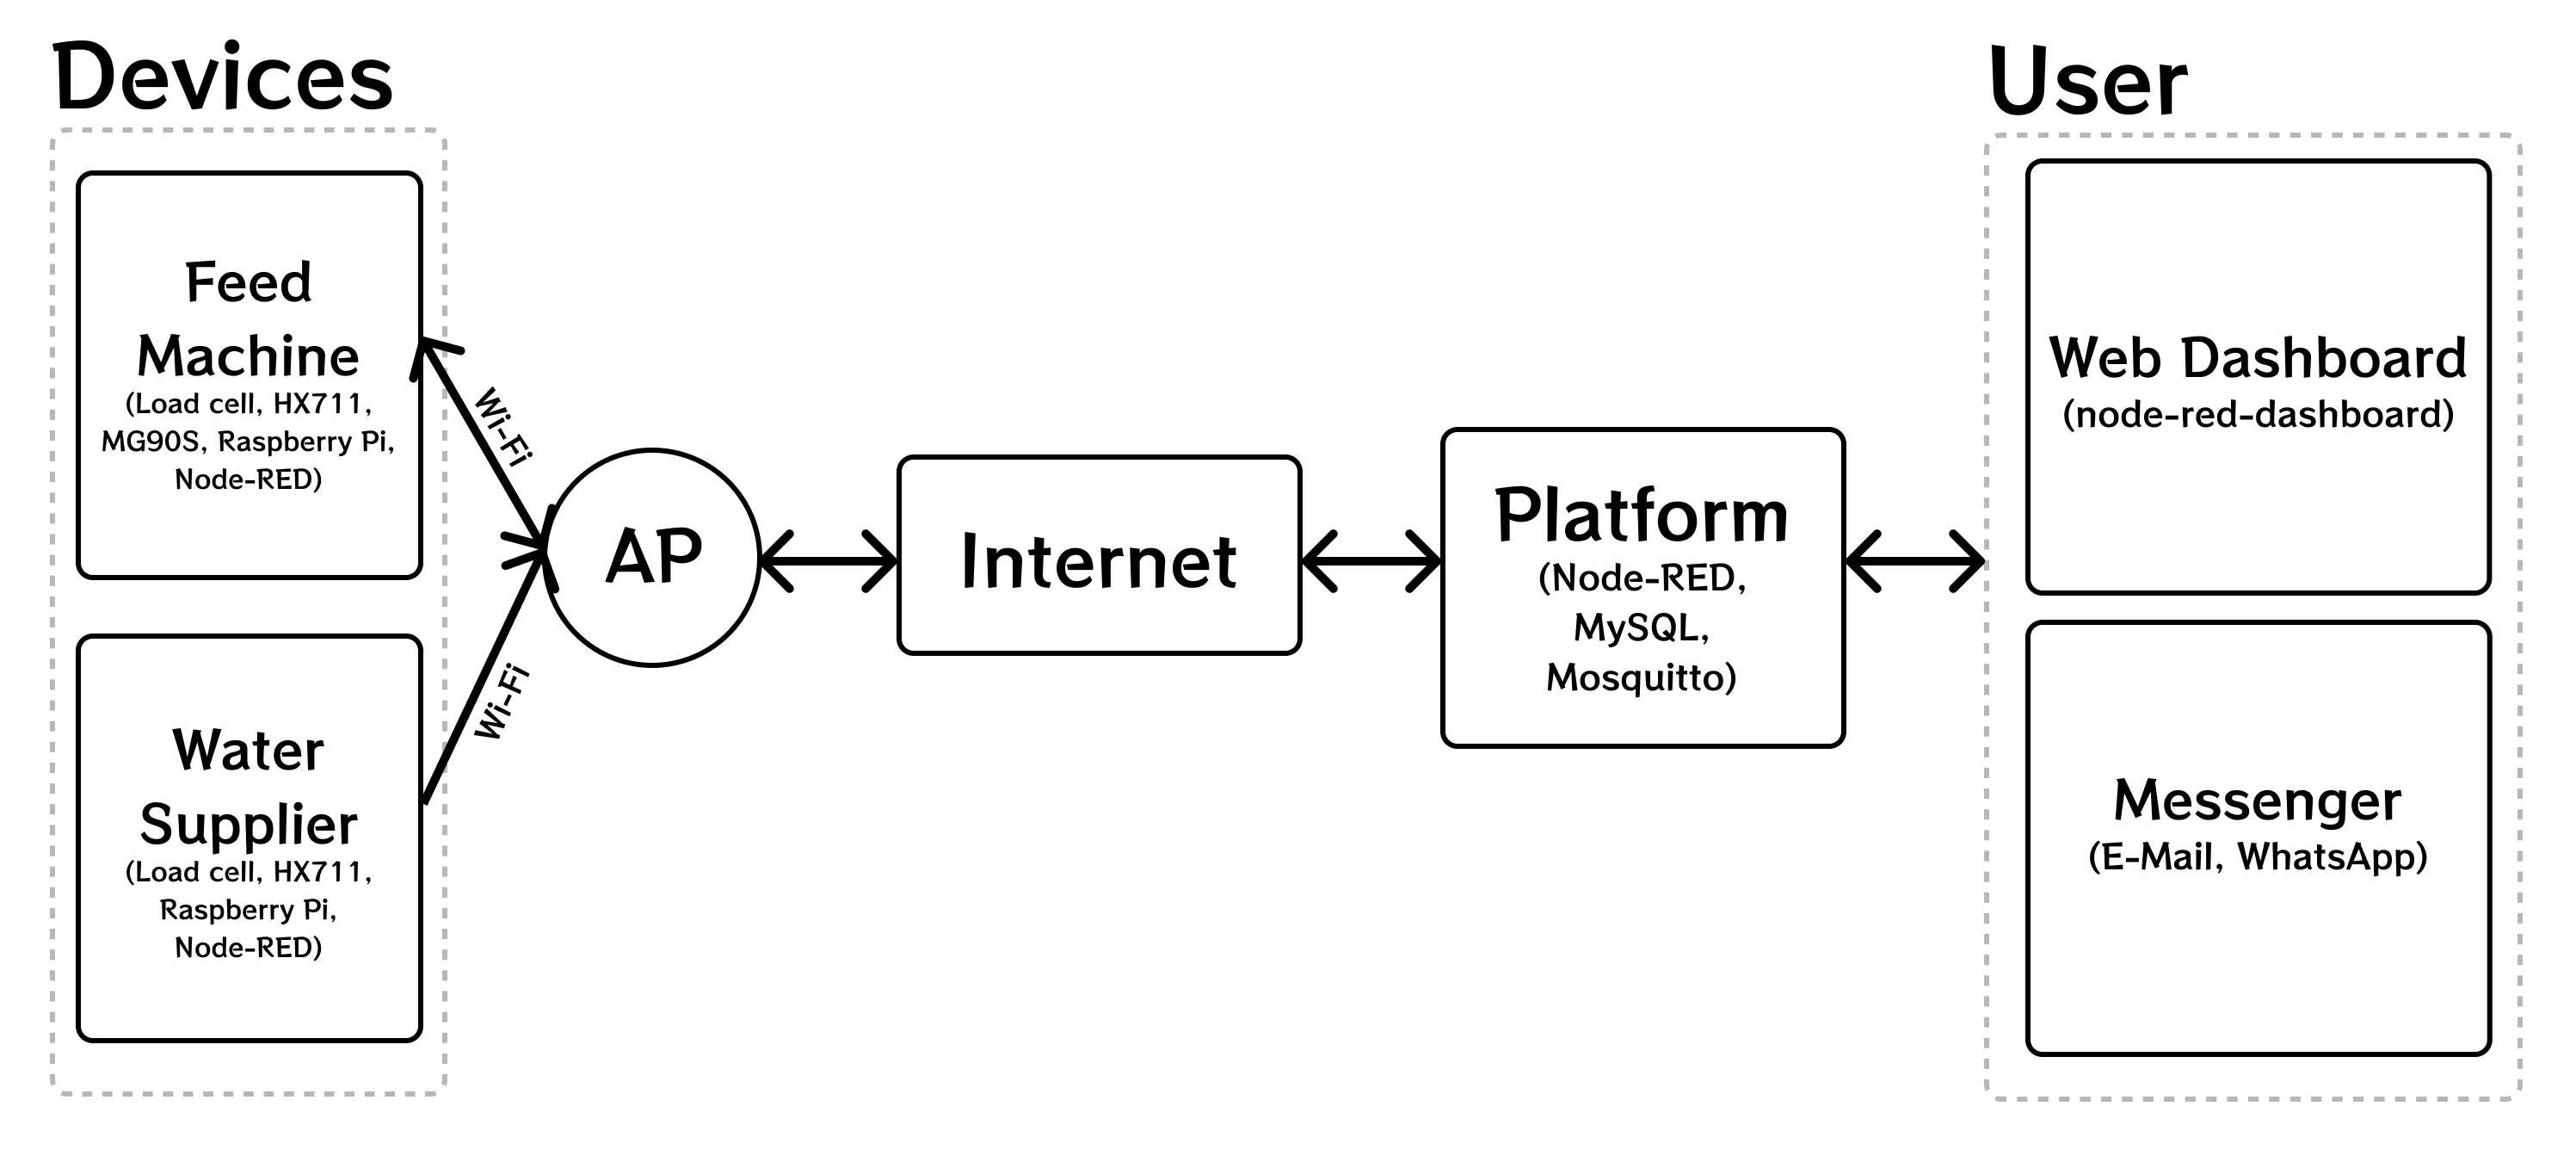
\includegraphics[width=0.5\textwidth]{./images/Overview.png}}
\caption{Petification overview}
\label{fig1}
\end{figure}

\section{Methodology}
The architecture of our proposed system is designed to connect the feed machine and water supplier with the user.
Each user and device can communicate in both directions through the platform.
The feed machine and water supplier are connected to an Access Point (AP) through Wi-Fi.
The messages published by the device are first sent to the AP via Wi-Fi and then to the platform via the internet.
The platform processes the messages and sends the processed data to the user in the form of web dashboard pages, emails, and WhatsApp messages.
Conversely, users can send requests to the platform through the web dashboard.
While some requests require only the platform, actuator activation requests are sent to the device with the help of the platform.
Fig. \ref{fig1} shows the overview of Petification.

\begin{figure}[htbp]
\centerline{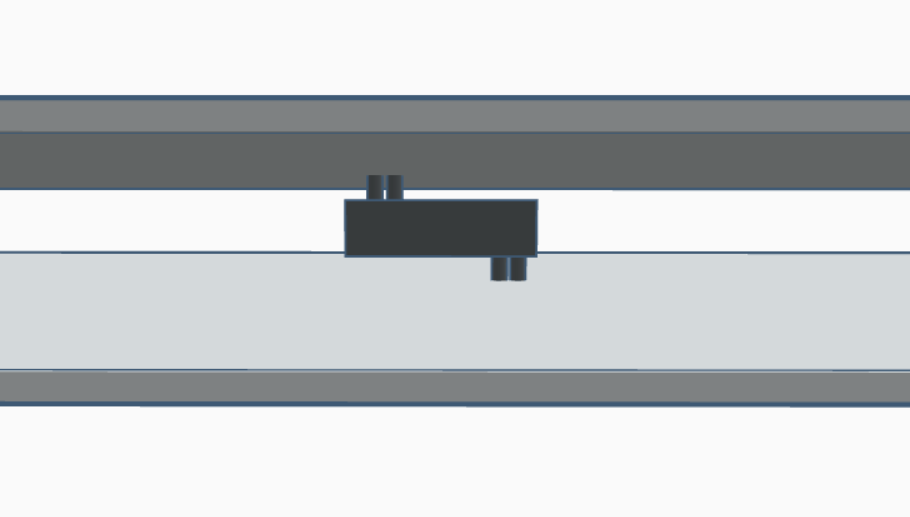
\includegraphics[width=0.3\textwidth]{./images/load-cell.png}}
\caption{Installaion of a load cell}
\label{fig2}
\end{figure}

\subsection{Water Supplier}
Weighing of water is performed with a single load cell that scales up to 5 kg with an accuracy of 1 g. A 500 mL water bottle used with an actual weight of 500 g is measured 500 times to obtain a reference unit during the calibration process.
As shown in Fig. \ref{fig2} the load cell is installed between the two plates to measure the pressure applied to the upper plate. And it is attached to the Raspberry Pi Zero W through the HX711 amplifier that  converts analog signals to digital signals. 
The calibration process was performed to obtain a reference unit for converting a measured value of a load cell into weight data.
The calibration formula is as follows:
%\[
\begin{equation}
   referenceUnit = \frac{average(loadCellMeasurements)}{actualWeight}
\end{equation}
%\]

%\begin{figure}[htbp]
%\centerline{\includegraphics[width=0.5\textwidth]{./images/watersuppliercircuit.jpg}}
%\caption{Circuit diagram of the water supplier}
%\label{fig3}
%\end{figure}

\begin{figure}[htbp]
\centerline{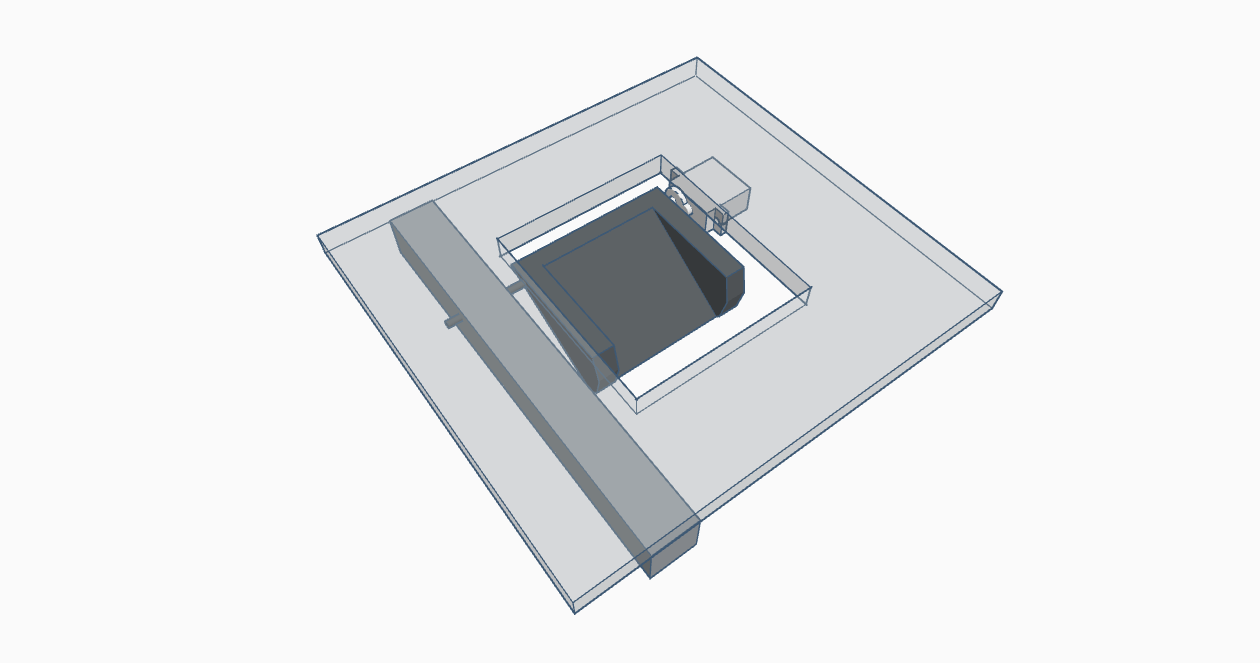
\includegraphics[width=0.5\textwidth]{./images/servo_gate.png}}
\caption{Food gate of the feed machine}
\label{fig4}
\end{figure}

\begin{figure}[htbp]
\centerline{\includegraphics[width=0.5\textwidth]{./images/feedmachinecircuit.jpg}}
\caption{Circuit diagram of the feed machine}
\label{fig5}
\end{figure}

\subsection{Feed Machine}
To weigh food, two load cells with HX711 amplifiers are installed under the food bowl and container in the same way as the water supplier.
In order to provide food to pets, a MG90S servo motor is mounted on the feed machine to control the food gate.
As shown in Fig. \ref{fig4}, the food gate has an open/close type. When the food gate opens, food is served to pets in a way that food rolls down the slope.
A load cell with an amplifier and an MG90S servo motor are attached to the Raspberry Pi Zero W as shown in Fig. \ref{fig5}.
% TODO: refine this sentence

\begin{figure}[htbp]
\centerline{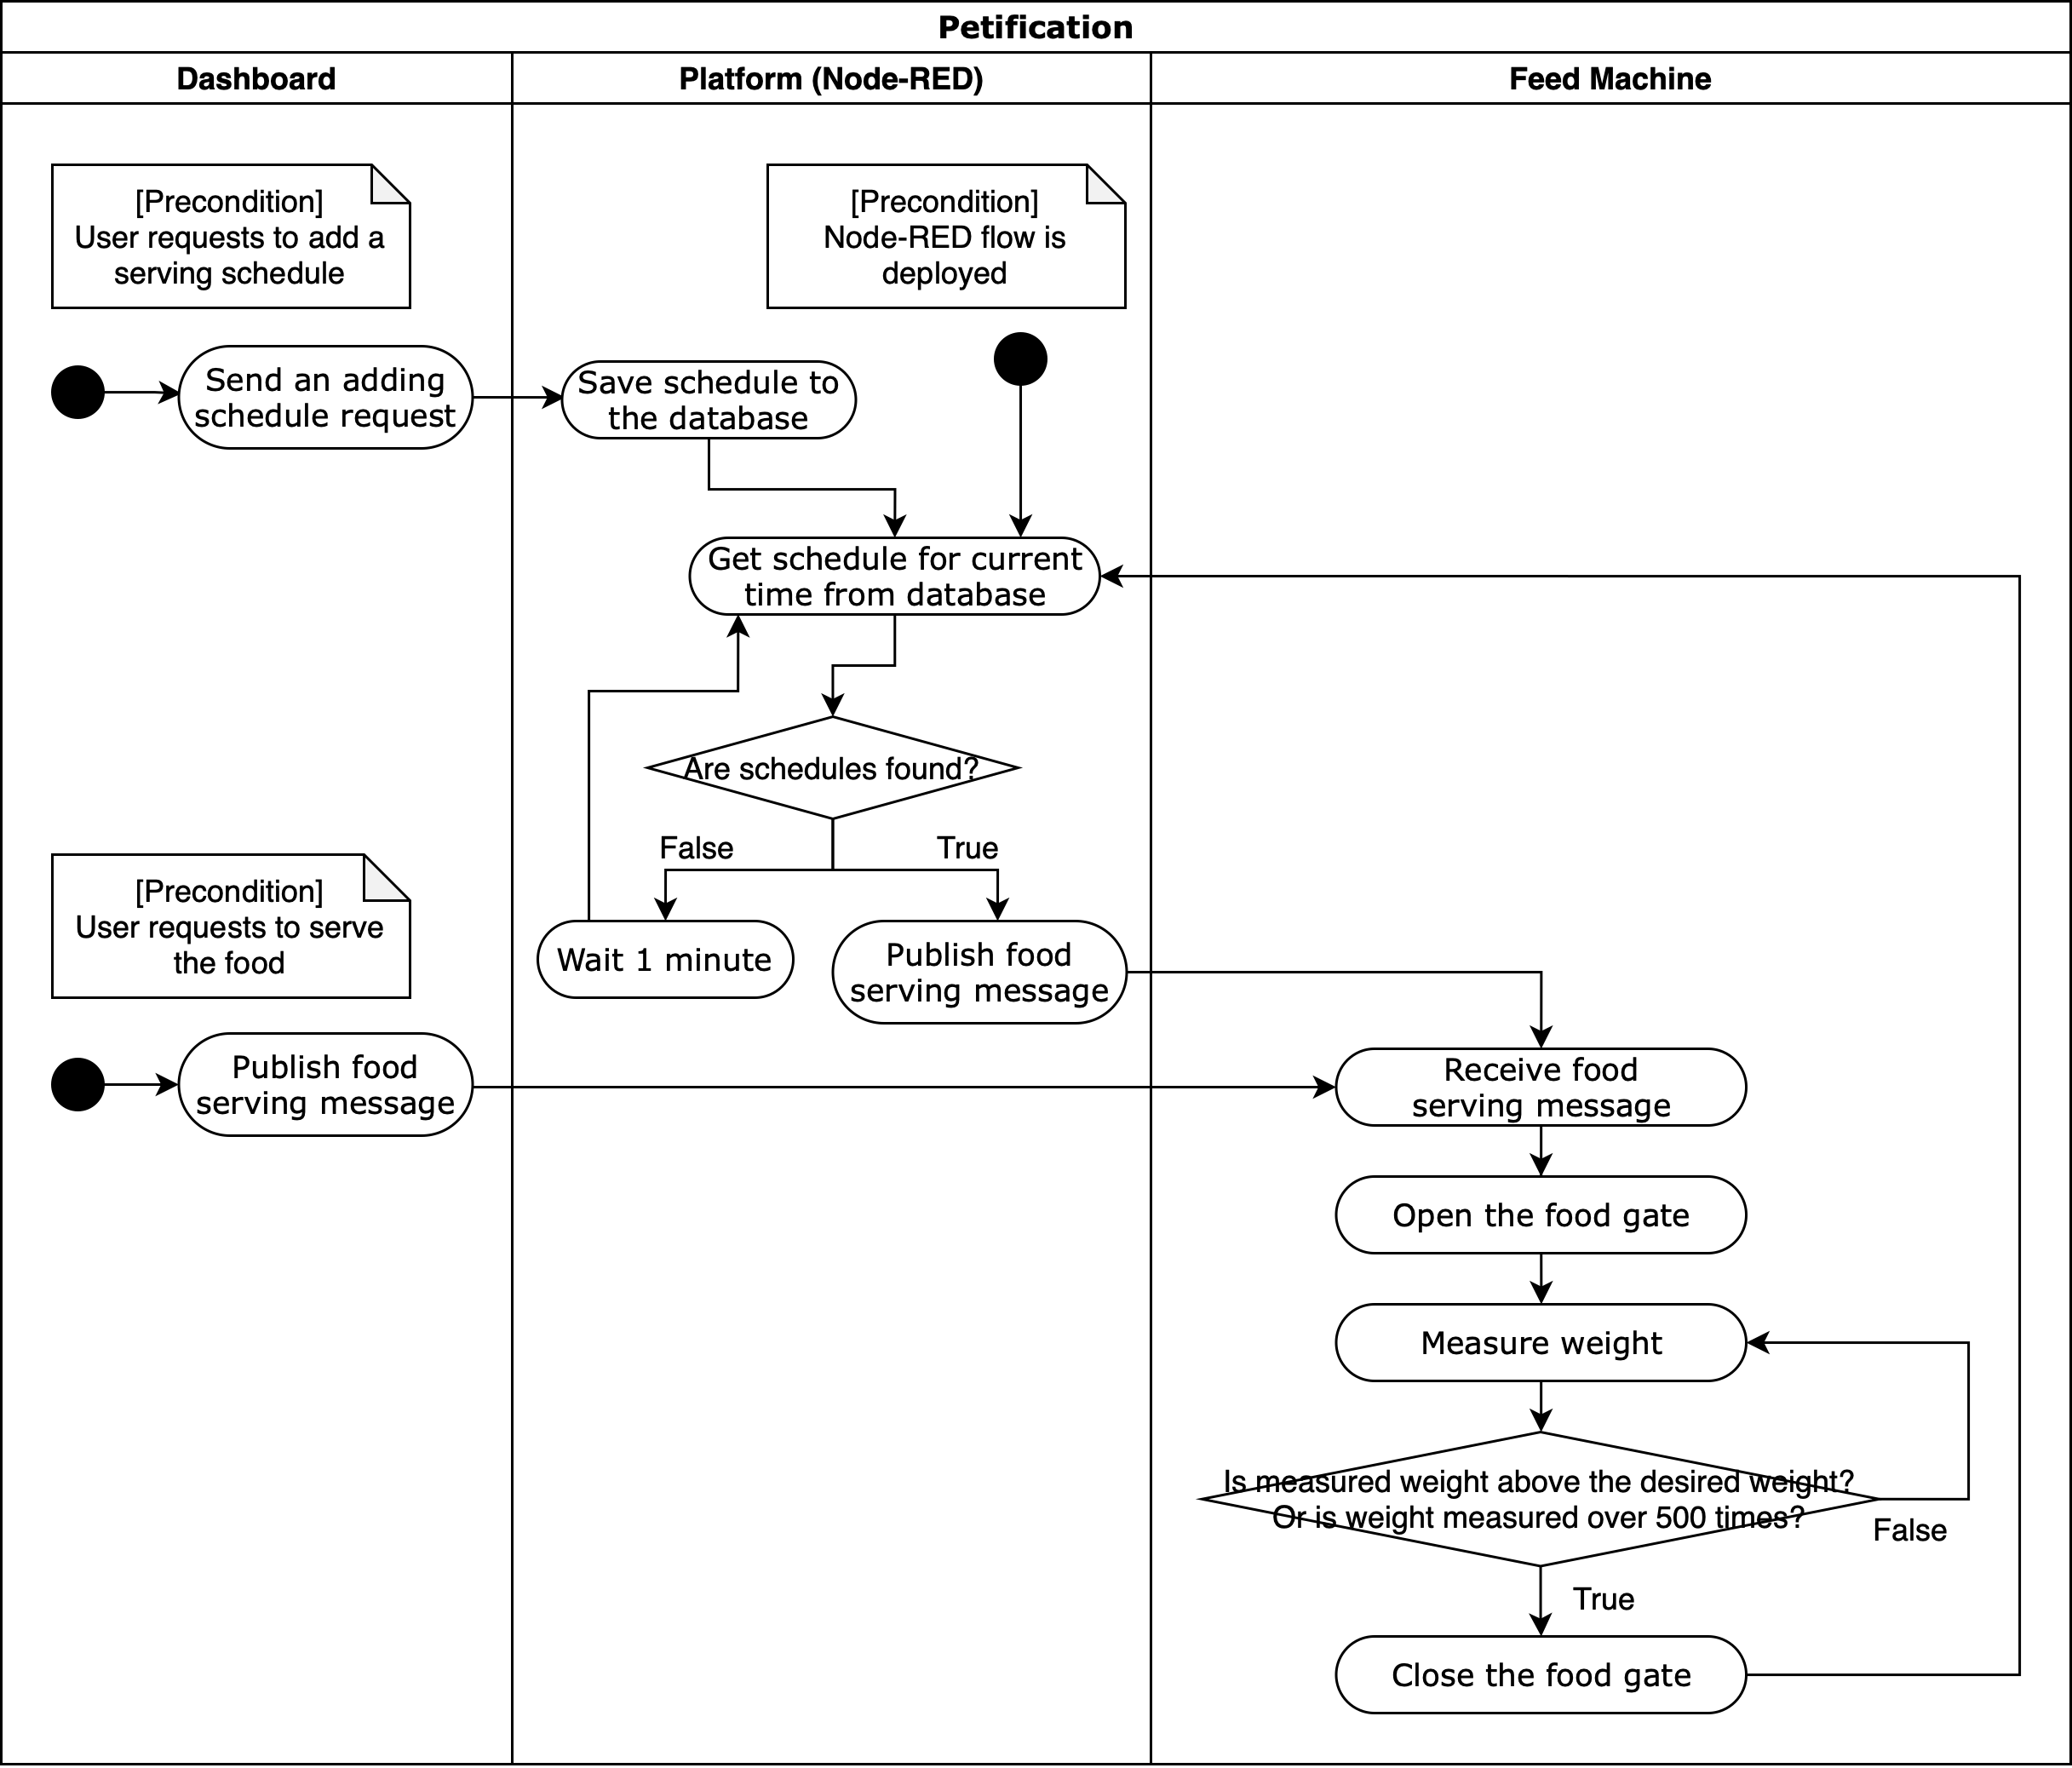
\includegraphics[width=0.5\textwidth]{./images/user2device.png}}
\caption{Activity diagram for user-to-device communication}
\label{fig6}
\end{figure}

\subsection{IoT Platform}
User-to-device communication occurs when the user remotely serve food to the pet, and device-to-user communication occurs when information and notification to the user are provided.
To send food serving message, the user can either set the serving schedule or press the button in the dashboard.
The serving schedules are stored in the database and checked every minute to serve the food when the scheduled time arrives.
After the feed machine receives the message, it opens the food gate and repeatedly scales the food bowl to serve the desired amount of food to the pet.
The detailed flow for the food serving is shown in Fig. \ref{fig6}.

\begin{figure}[htbp]
\centerline{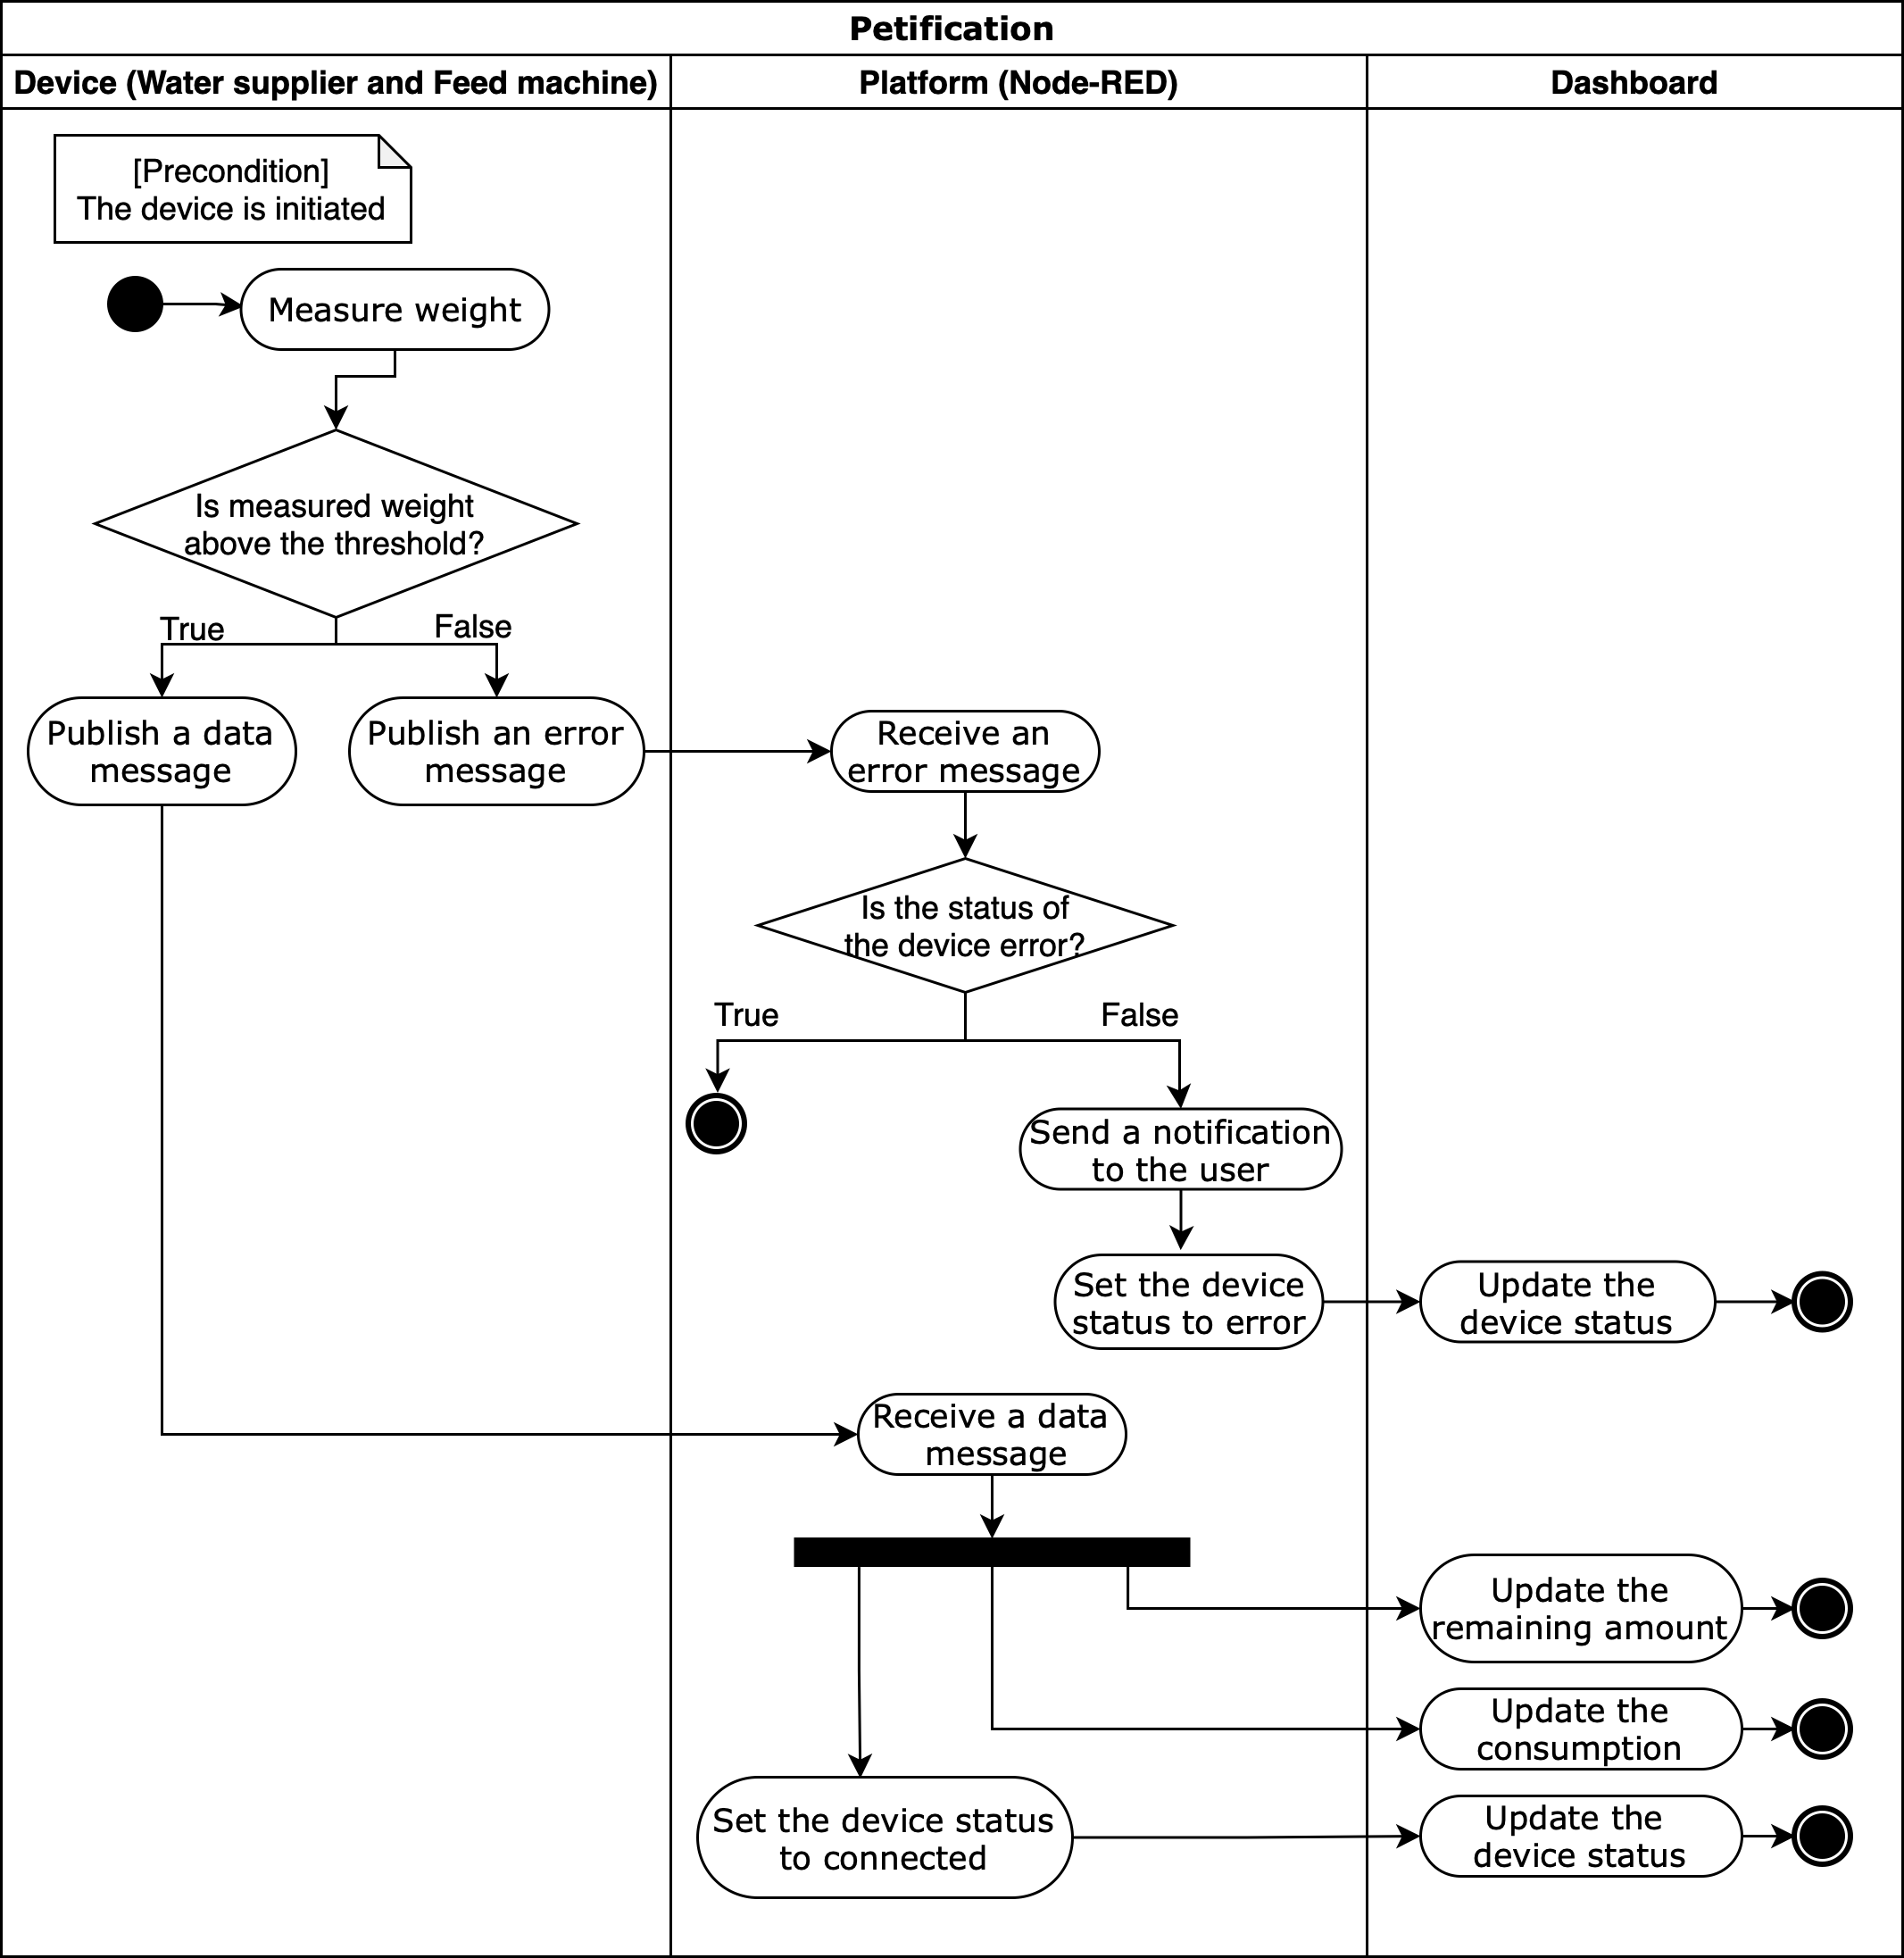
\includegraphics[width=0.5\textwidth]{./images/device2user.png}}
\caption{Activity diagram for device-to-user communication}
\label{fig7}
\end{figure}

\begin{algorithm}
\caption{Calculate consumption}\label{algo1}
\begin{algorithmic}
    \Procedure{CalcConsumption}{}
        \State $prevConsumption \gets \text{previous } \textit{consumption}$
        \State $currScale \gets \textit{scale} \text{ of received message}$
        \State $prevScale \gets \textit{scale} \text{ of  previous record}$
        \State $decrease \gets 0$
        \If{$precScale \neq \textit{null} \And prevScale > currScale$}
            \State $decrease \gets prevScale - currScale$
        \EndIf
        %\Return {$prevConsumption + decrease$}
        \State \textbf{return} $prevConsumption + decrease$
    \EndProcedure
\end{algorithmic}
\end{algorithm}

The device weighs food and water to provide information and alerts to the user. 
If the measured weight exceeds the threshold value of 10 g, a message containing the measured weight is sent to the platform. 
These data messages are used to update and display the balance, consumption and device status to the user.
However, if the measured weight is below a threshold, an error message is sent to the platform to update the device status and inform the user that food or water is empty.
Fig. \ref{fig7} shows the detailed device-to-user flow and Algorithm \ref{algo1} shows the pseudocode for calculating consumption.

Three open-source projects are used for the platform: Node-RED, Eclipse Mosquito, and MySQL. 
\subsubsection{Node-RED}
Node-RED is a flow-based, open-source visual development tool that makes it easy for developers and non-developers to develop programs \cite{b12}.
One of Node-RED's strengths is its powerful community; Various nodes such as dashboard widgets and database drivers are being deployed through the Node Package Manager (NPM).
Another advantage is that it can be run in a variety of environments, including local, Raspberry Pi, Docker, and cloud instances.
Thus, Node-RED v2.2.1 is installed in the platform server as well as the Raspberry Pis in both water supplier and feed machine.

\subsubsection{Eclipse Mosquitto MQTT message broker}
MQTT is an OASIS standard protocol and provides a lightweight publish/subscribe messaging transport for IoT \cite{b8}.
The publish/subscribe model of the MQTT protocol allows IoT platforms to support bidirectional communication in such a way that by subscribing to a topic of a message, others can receive messages published to that topic.
In this study, Eclipse Mosquitto v1.4.15 is used as the MQTT message broker, an open-source implementation of the MQTT protocol 5.0, 3.1.1 and 3.1 versions \cite{b13}.

\subsubsection{MySQL}
MySQL is a fast, flexible, and easy-to-use open-source database with a relational database management system (RDBMS).
In addition to performance and security aspects, MySQL is considered a suitable database for managing effective data flow because of its compatibility with Node-RED.
And MySQL v5.7.37 is integrated as a component of the platform.
%\begin{figure}[htbp]
%\centerline{\includegraphics[width=0.5\textwidth]{./images/WaterSupplierErrorDetection.png}}
%\caption{Node-RED screenshot for publishing weight or error message}
%\label{fig8}
%\end{figure}
%\begin{figure}[htbp]
%\centerline{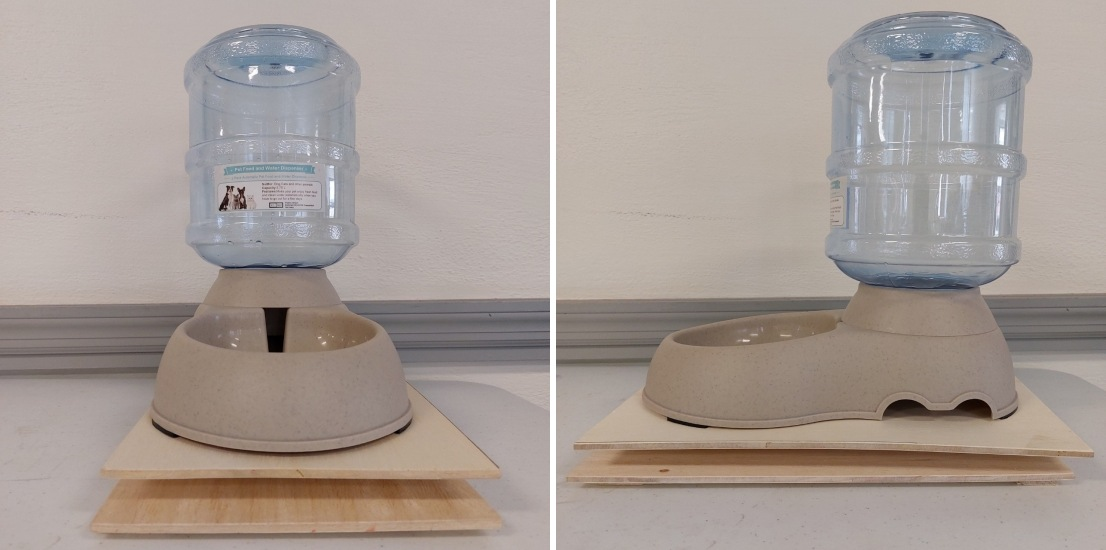
\includegraphics[width=0.5\textwidth]{./images/water-supplier.jpg}}
%\caption{Result of implementation for water supplier}
%\label{fig9}
%\end{figure}

\section{Implementation and Result}
\subsection{Water supplier}
Calibrating and measuring the weight of water is done in python code.
Measurement results are available in Node-RED using an exec node that can execute python code.

However, there is always a possibility of measurement error even if calibration is performed.
To reduce the measurement error after calibration, we used the smooth node of the non-red-node-smooth node module.
After weighing, the switch node determines if the weight is below a threshold to determine the type of message being sent (weighted data or error).
The messages are sent after the function node prepares the message and the "mqtt out" node publishes the message.
%The Node-RED flow for publishing weight or error messages is shown in Fig. \ref{fig8} and 
%The implemented water supplier is shown in Fig. \ref{fig9}.

%\begin{figure}[htbp]
%\centerline{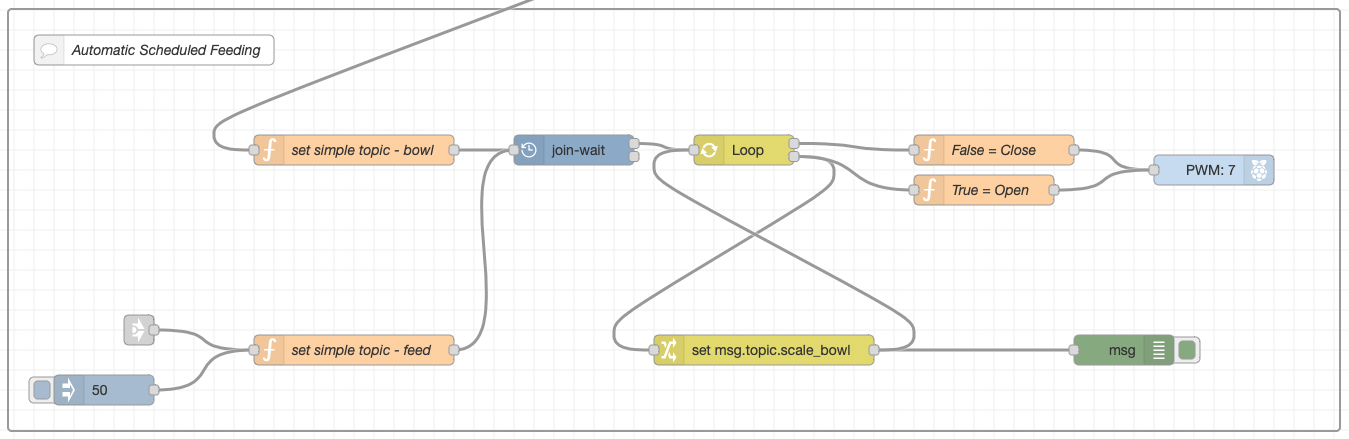
\includegraphics[width=0.5\textwidth]{./images/automaticFeeding.png}}
%\caption{Node-RED screenshot for automatic feeding}
%\label{fig10}
%\end{figure}

%\begin{figure}[htbp]
%\centerline{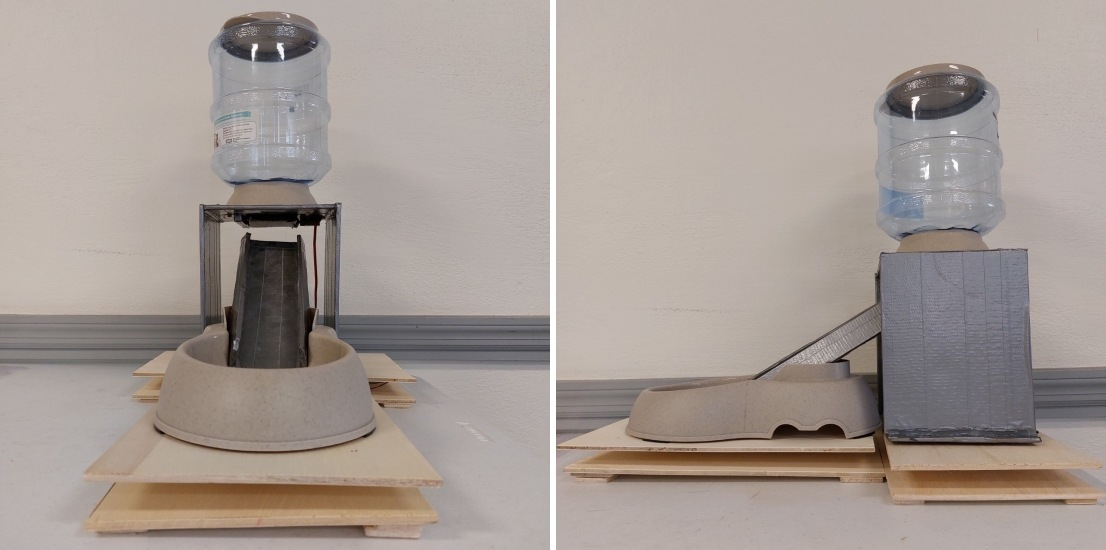
\includegraphics[width=0.5\textwidth]{./images/feed-machine.jpg}}
%\caption{Result of implementation for feed machine}
%\label{fig11}
%\end{figure}

\begin{figure}[htbp]
\centerline{\includegraphics[width=0.5\textwidth]{./images/FoodnWaterSupplier.jpg}}
\caption{Water supplier(left) and Feed machine(right)}
\label{fig11new}
\end{figure}

\subsection{Feed machine}
It implements a flow to provide a certain amount of food in addition to the weighing flow, which is similar to a water supplier. 
The food serving flow starts after a message arrives containing the desired serving amount as the message payload.
The join-wait node in the node-red-contrib-join-wait node module waits for a food serving message and returns an object after the message arrives.
Then, the current weight is repeatedly measured and compared by the loop node from the node-red-contrib-loop-processing and change node.
The food gate opens on the first loop and closes when the current weight is above the desired weight or the loop is repeated 500 times.
Open and close using the pi-gpiod out node of the node-red-node-pi-gpiod node module. 
%The Node-RED flow for food serving is shown in Fig. \ref{fig10} and the implemented feeder is shown in Fig. \ref{fig11}.
Both feed machine and water supplier are implemented shown in Fig. \ref{fig11new}.

\subsection{IoT Platform}
%The Petification platform uses cloud instances for deployment.
Mosquitto, MySQL, and Node-RED are installed on the cloud instance, and the firewall, DNS, and certificate for TLS/SSL communication are configured for networking.
In Node-RED, seven IoT platform components are implemented as seven flows.
%A screenshot of the implemented Node-RED flow is shown in Fig. \ref{fig12}.

%\begin{figure}[htbp]
%\centerline{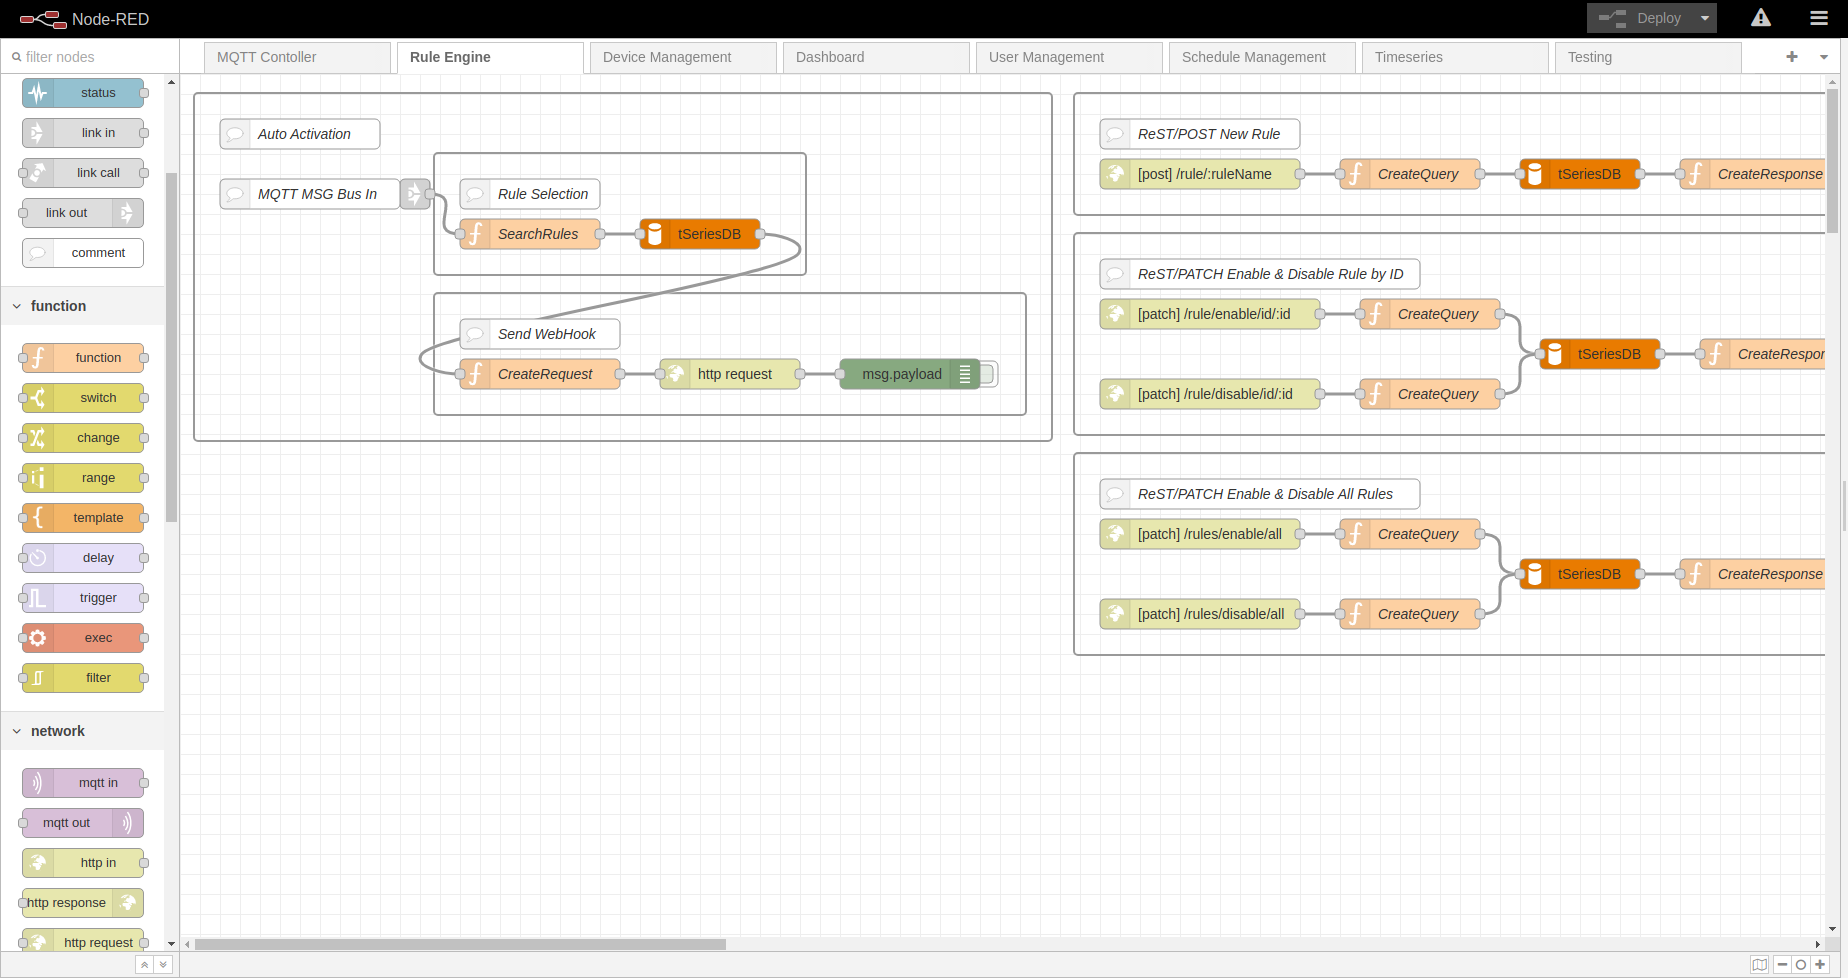
\includegraphics[width=0.5\textwidth]{./images/node-red-platform-screenshot.png}}
%\caption{Node-RED flow screenshot of IoT platform}
%\label{fig12}
%\end{figure}

\subsubsection{MQTT Controller}
The MQTT controller flow on Node-RED is the gateway for MQTT messages to go to Node-RED.
The main purpose of this flow is to parse the topic and payload of the incoming MQTT message to provide useful information such as the MQTT username and client ID to other flows.
The mqtt-in node is used to subscribe to and receive MQTT messages, and the function node is used to parse the message and transform it into an object.

\subsubsection{Rule Engine}
The purpose of the Rule Engine is to activate actions based on MQTT messages.
Rule Engine's logic is inspired by "Building Your Own IoT Platform" \cite{b14}.
For every message published, the Rule Engine checks the rules table in the database to find a rule whose message pattern meets the message content.
The action corresponding to the rule is defined in the ReST API format, so the action is activated by sending an HTTP request.

\subsubsection{Device Manager}
The Device Manager flow is to handle devices attached to the platform.
It provides a ReST API to add new devices to the platform, modify the status of devices, and delete devices.
It also provides functionality for publishing food serving messages to specific devices.

\begin{figure}[htbp]
\centerline{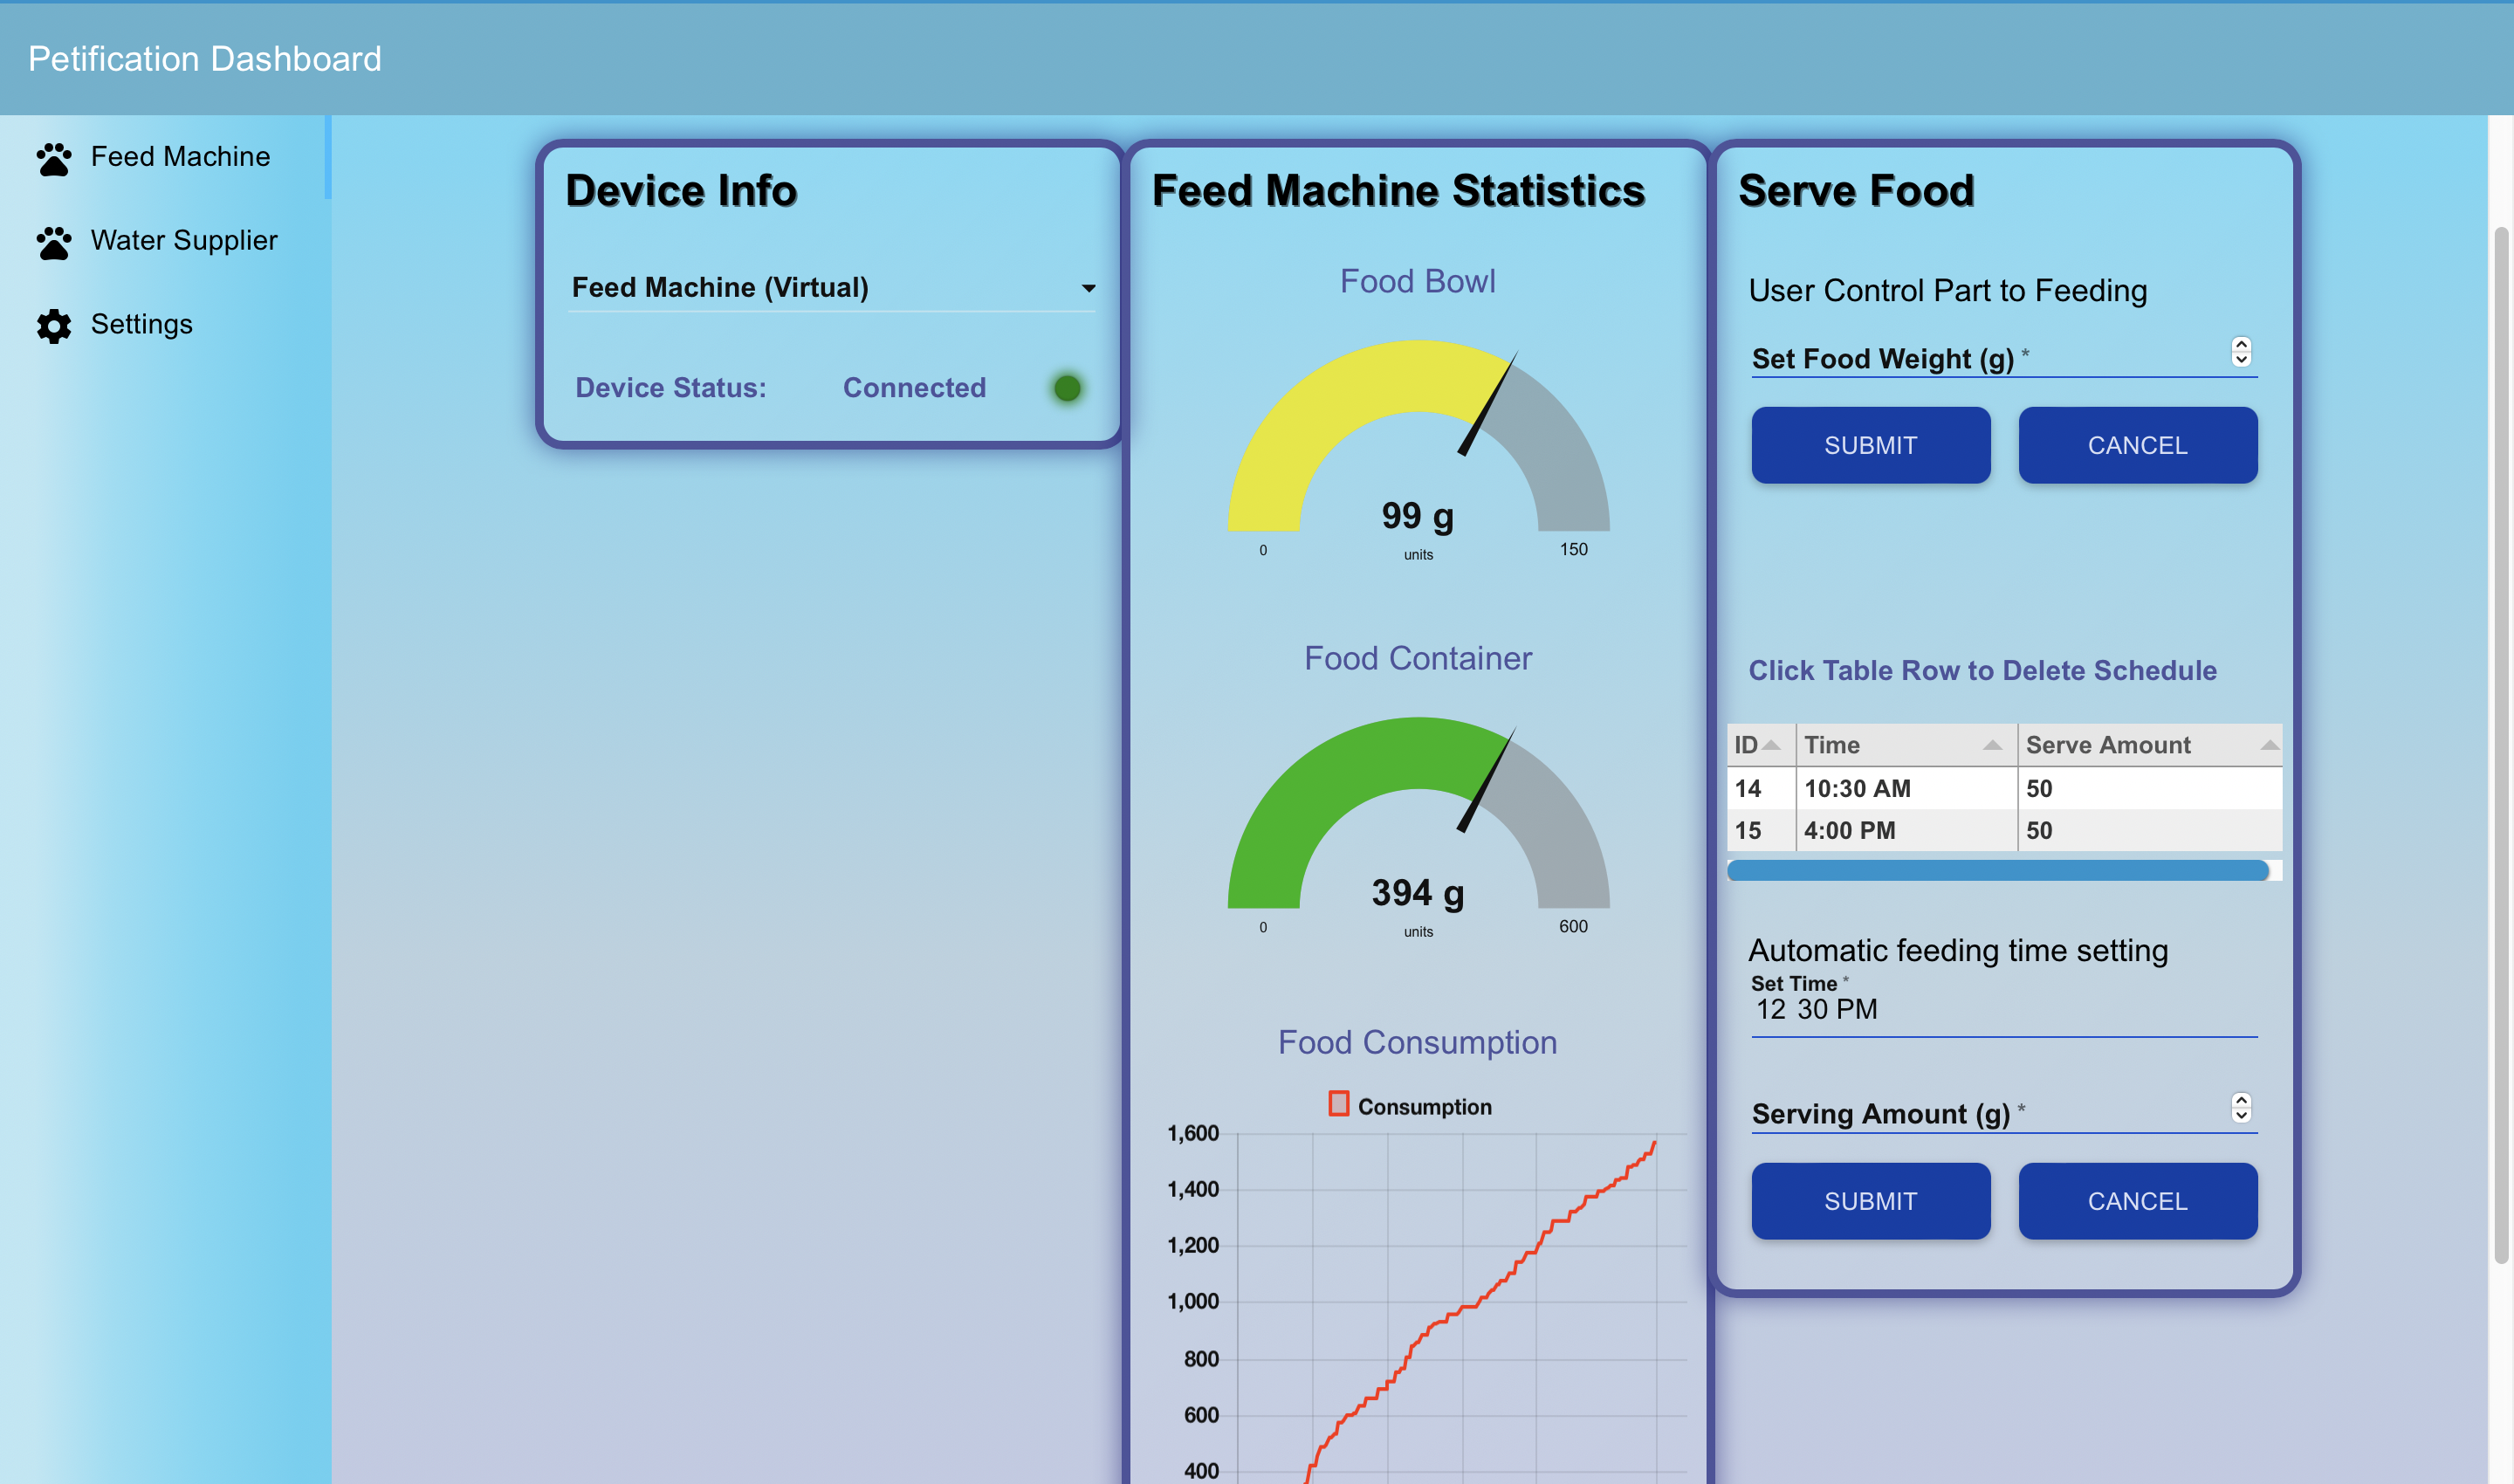
\includegraphics[width=0.45\textwidth]{./images/feed_machine_ui.png}}
\caption{Screenshot for Feed Machine tab of the dashboard}
\label{fig13}
\end{figure}

\begin{figure}[htbp]
\centerline{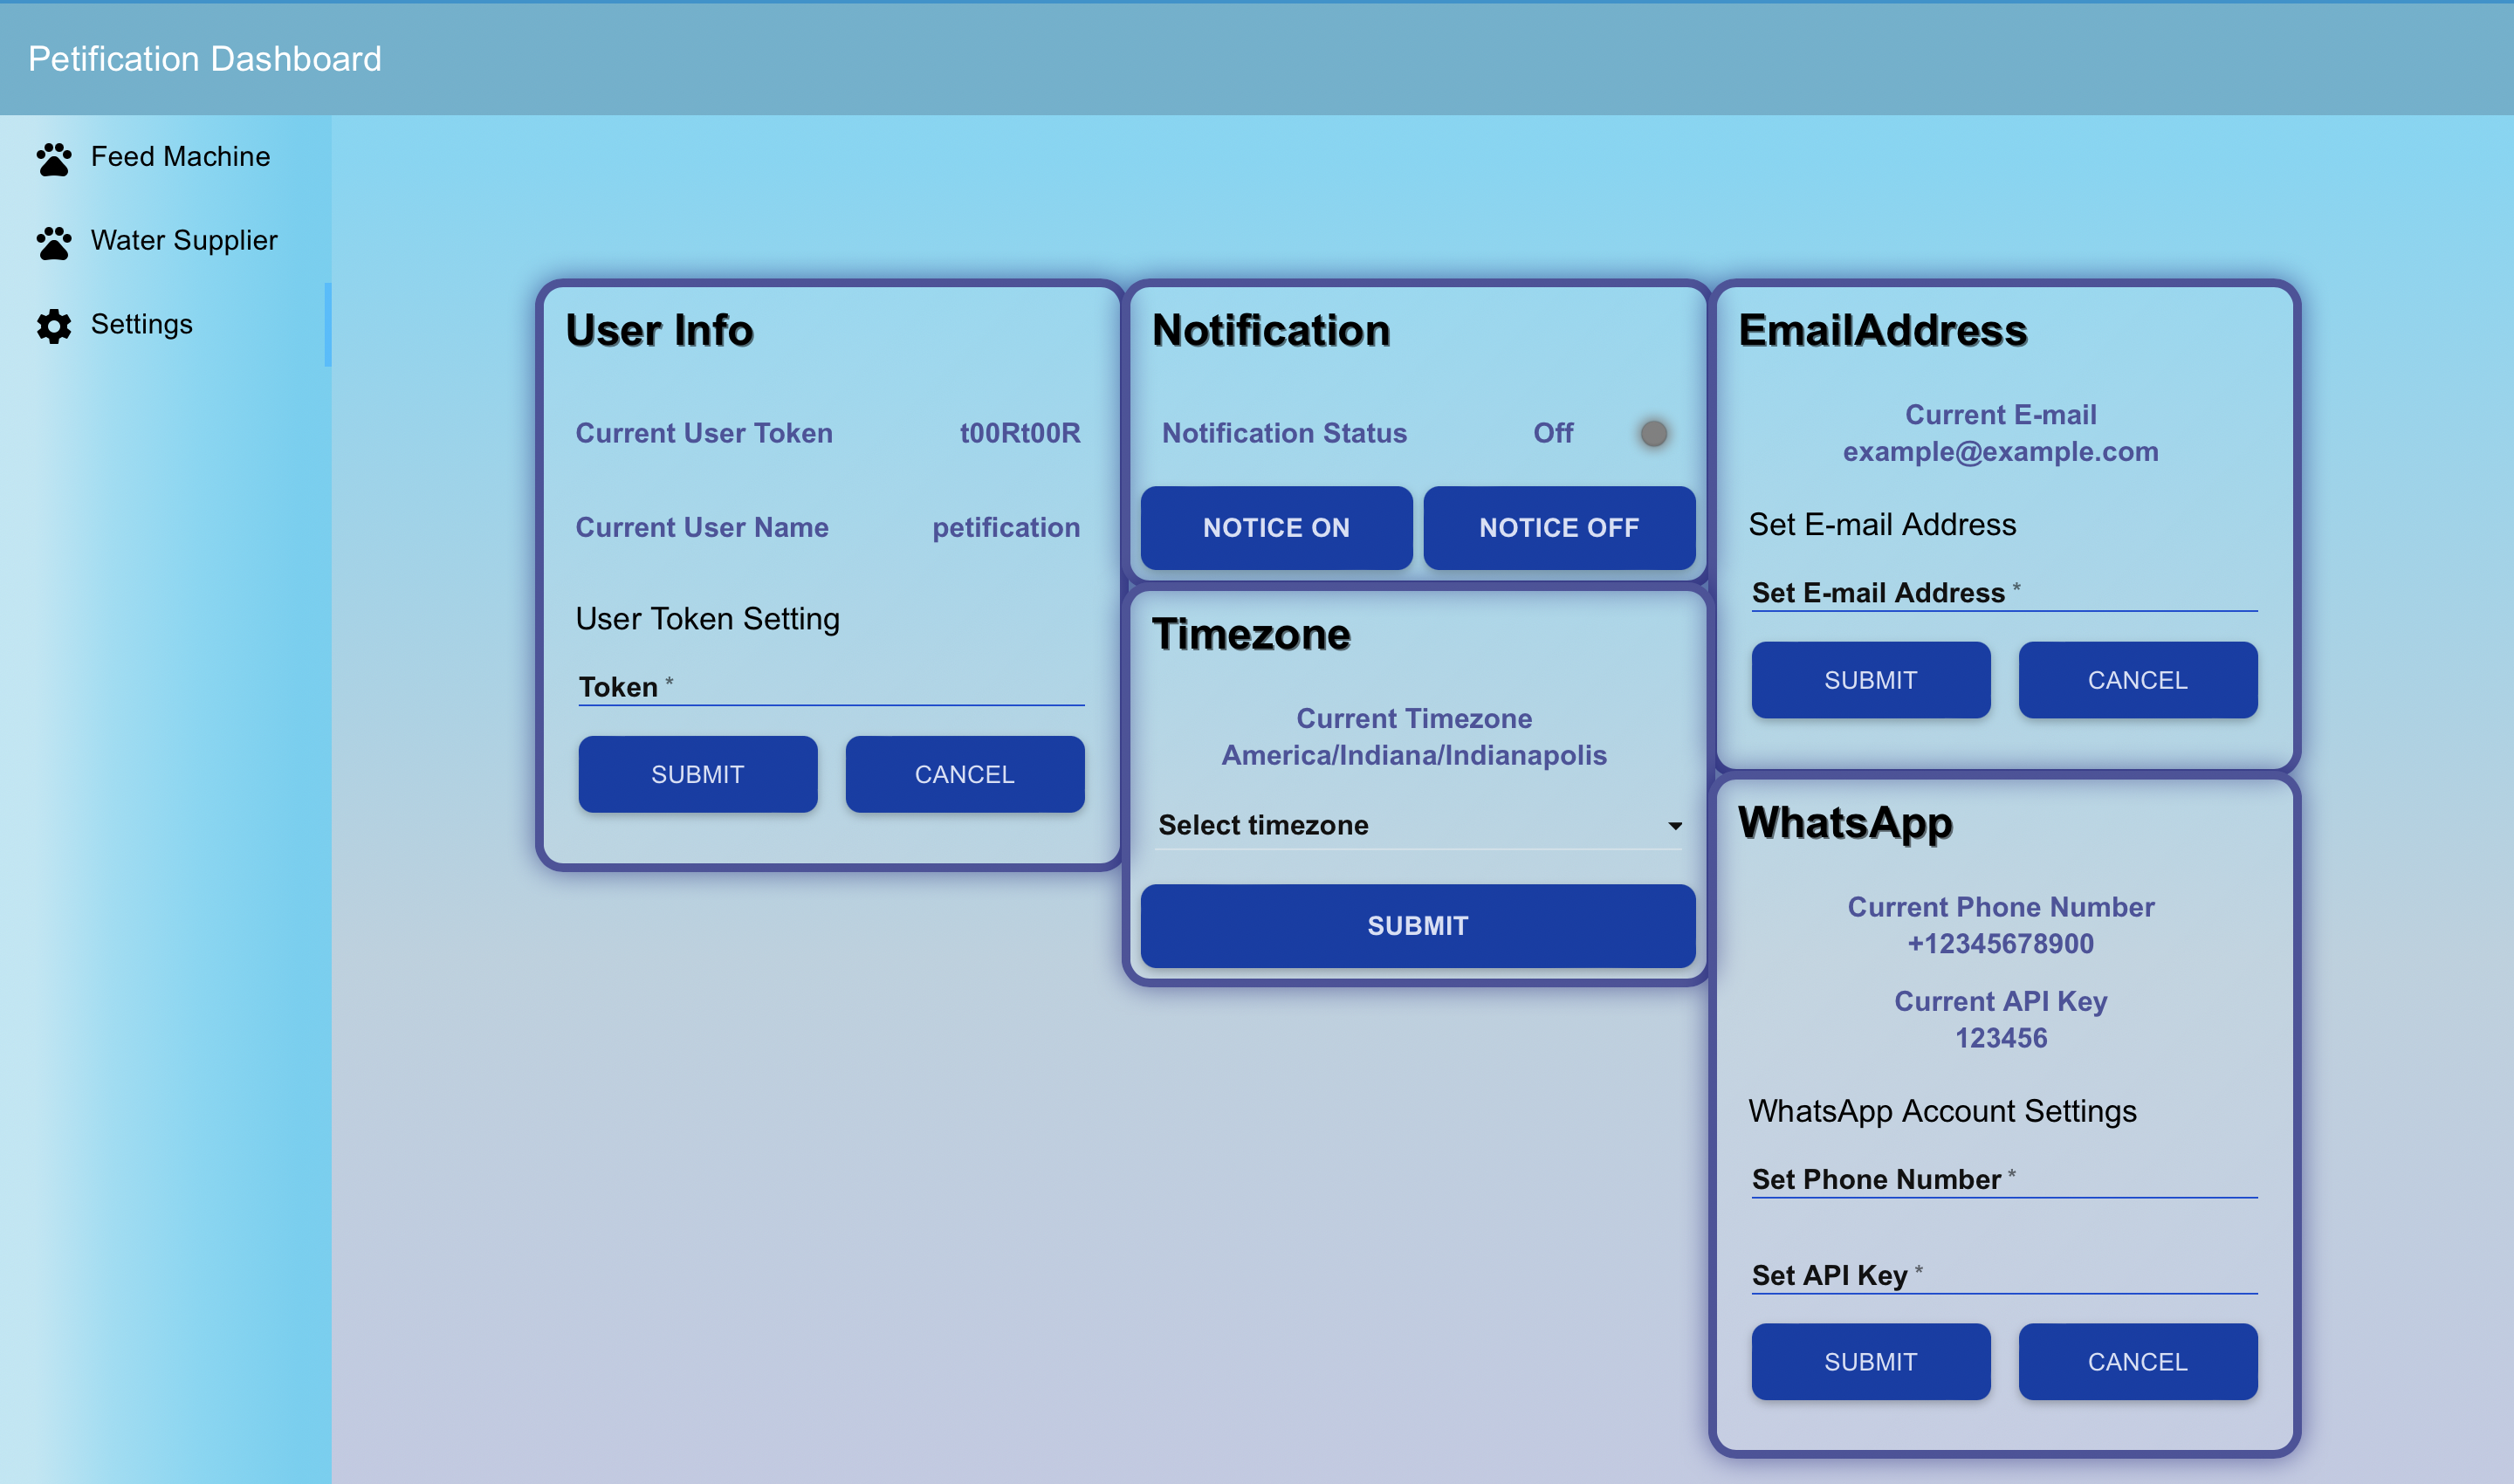
\includegraphics[width=0.45\textwidth]{./images/user_settings_ui.png}}
\caption{Screenshot for User Setting tab of the dashboard}
\label{fig13a}
\end{figure}

%\begin{figure}[htbp]
%\centerline{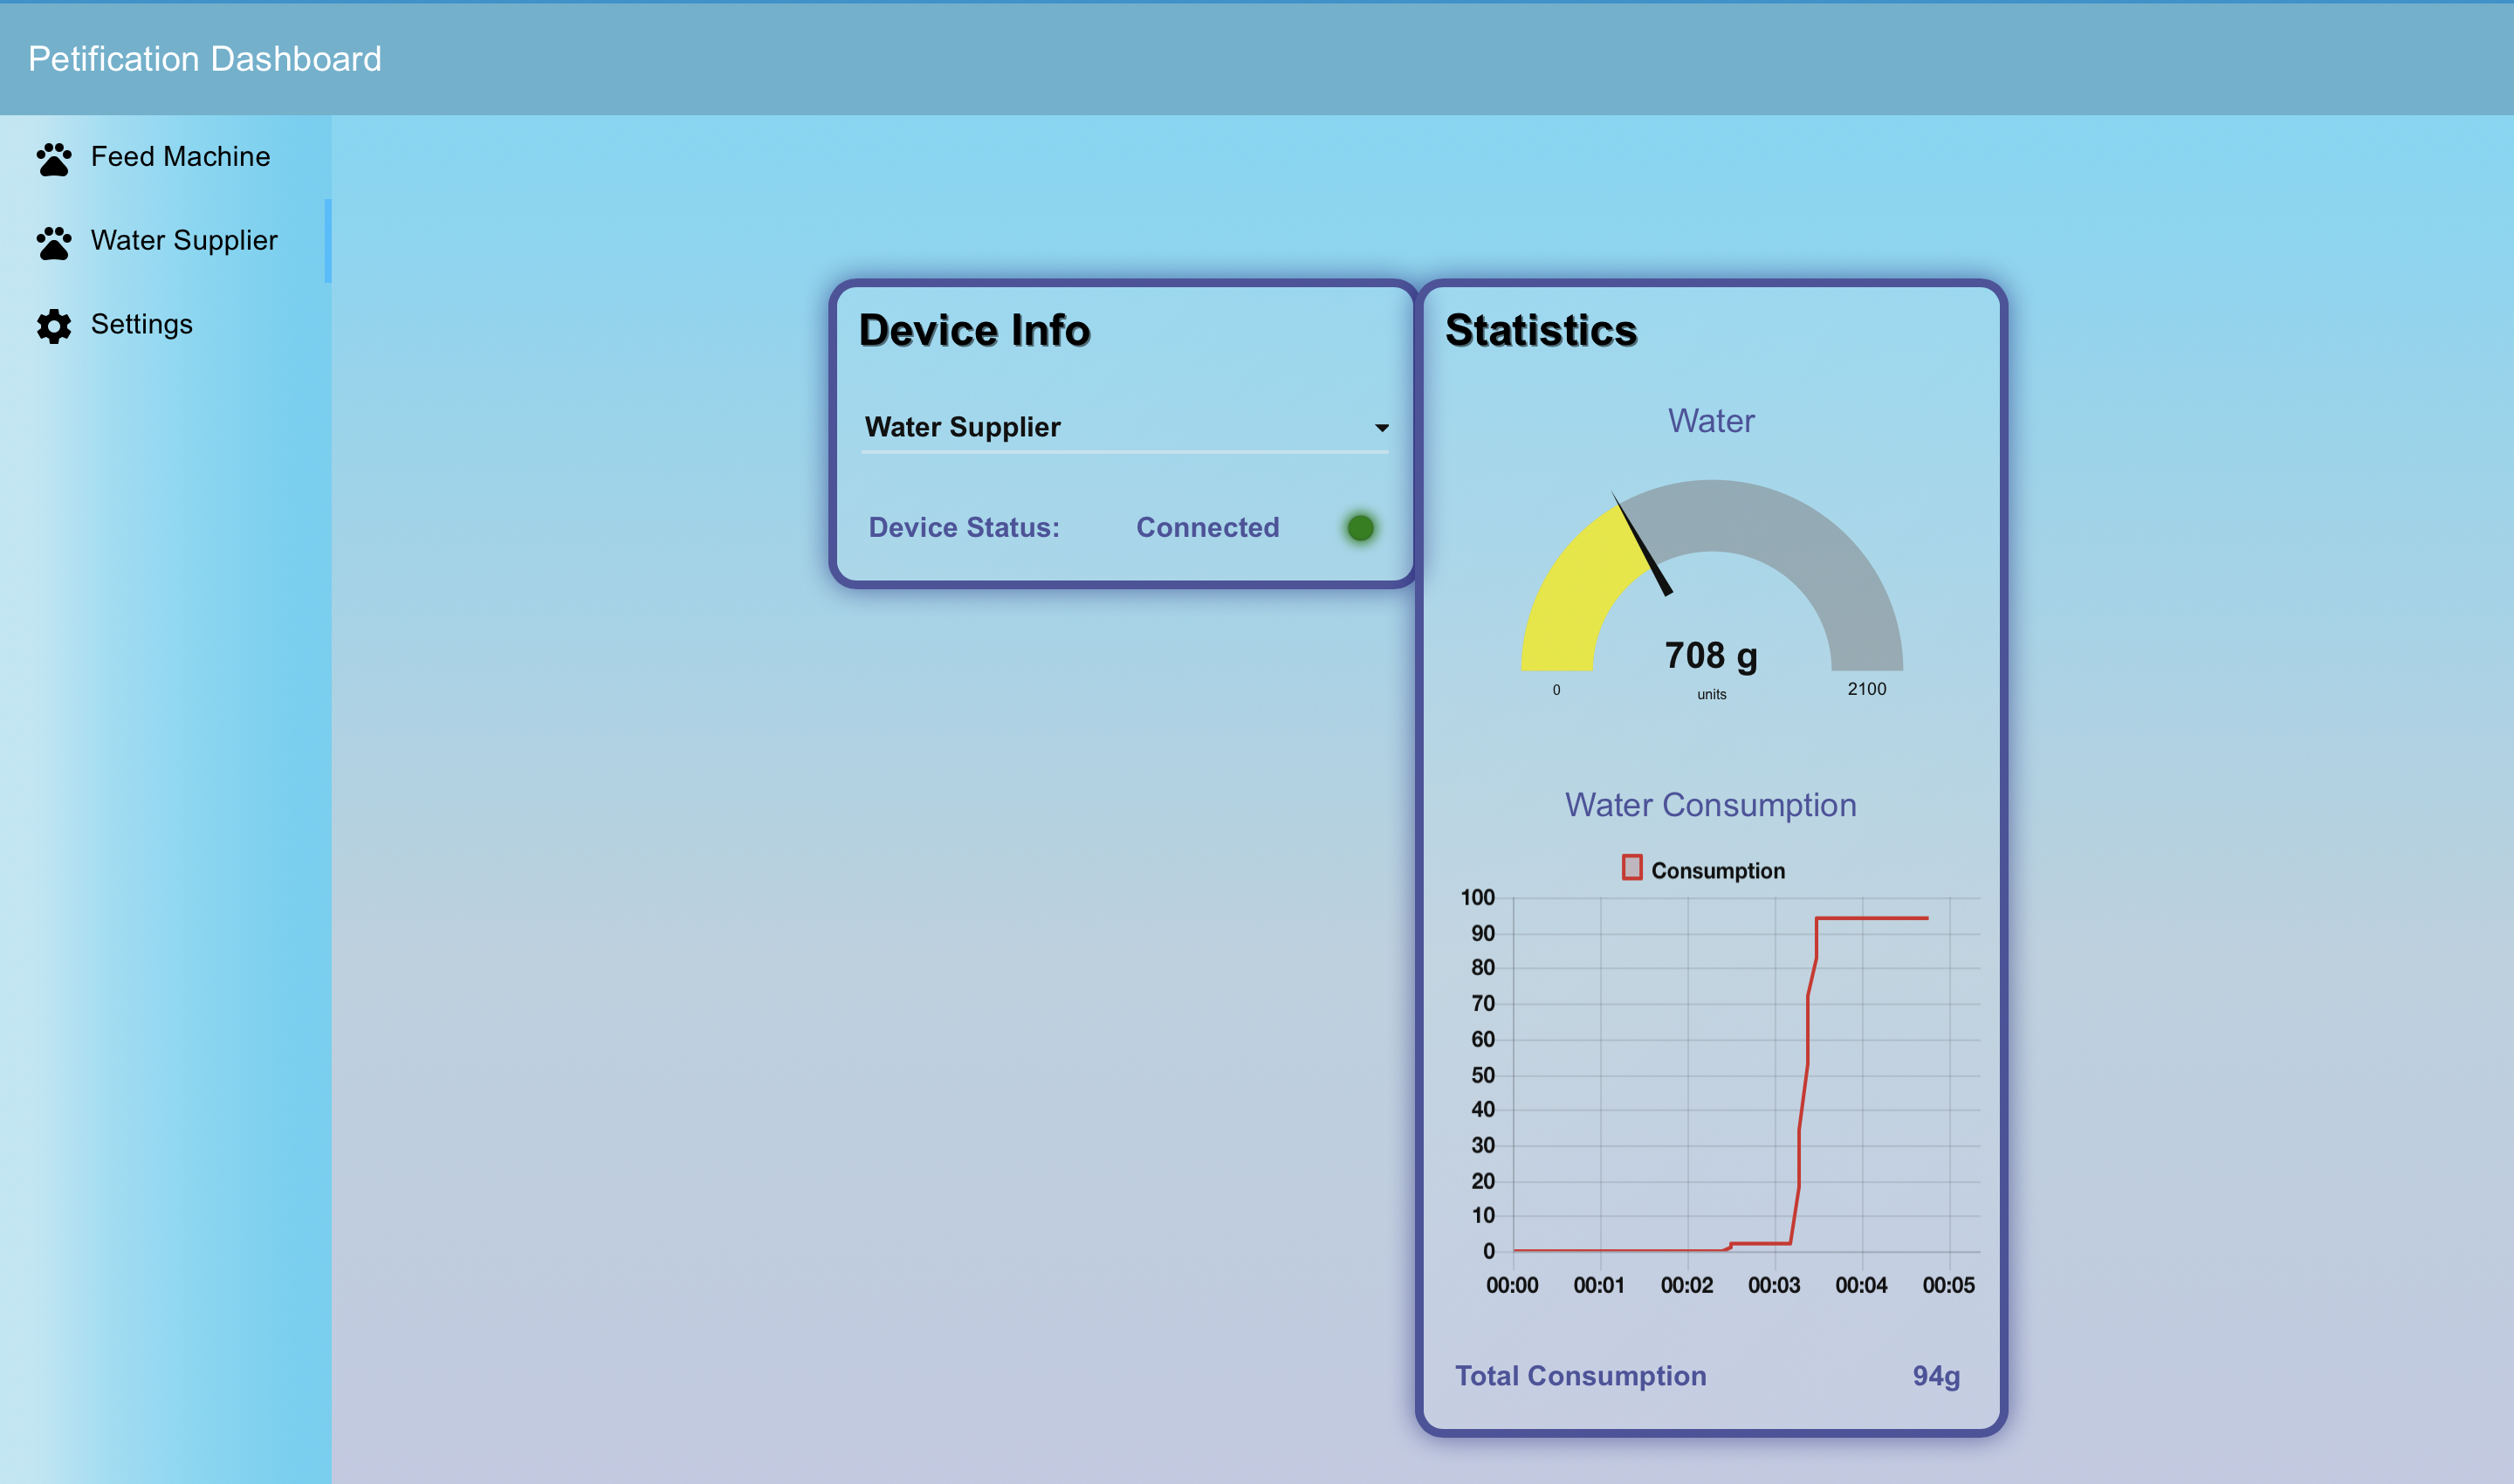
\includegraphics[width=0.5\textwidth]{./images/water_supplier_ui.png}}
%\caption{Screenshot for Water Supplier tab of the dashboard}
%\label{fig13b}
%\end{figure}

\subsubsection{Dashboard}
This provides users with a graphical user interface (GUI). The dashboard consists of three tabs: Feed Machine tab, Water Supplier tab, and User Settings tab.

\begin{itemize}
\item{\it{Feed Machine Tab:}}
Under the Feed Machine tab, Device Information widget, Feed Machine Statistics widget, and Serve Food widget are provided. 
As all the functionalities this tab provides are device specific, selecting a device is included in the Device Information widget and is displayed as a dropdown.
%The status for the selected device is provided in the text and LED-shaped icon.
The Feed Machine Statistics widget provides leftover food and food consumption. The amount of leftover is displayed in a gauge and food consumption is displayed in a line graph. Users can check all the feeding schedules in the table format, add a new schedule by user input interface, and delete the existing schedule by clicking the row of the table. Fig. \ref{fig13} shows the Feed Machine tab on the Dashboard.
\item{\it{Water Supplier Tab:}}
Similar to the Feed Machine tab, the Water Supplier tab provides two widgets: Device Information widget and Water Supplier Statistics widget. The mechanism for each widget is identical to the Feed Machine tab. 
\item{\it{User Settings Tab:}}
The User Settings tab provides five widgets: User Information, Timezone settings, Notification settings, E-Mail address settings, and WhatsApp settings. 
Notification settings, E-Mail address settings, and WhatsApp settings widgets are to control error notification. Users can turn notifications on or off with the Notification settings widget and decide which accounts receive email and WhatsApp messages. Fig. \ref{fig13a} shows the screenshot of the implemented User Settings tab.
\end{itemize}

\subsubsection{User Management}
The user managing flow is to provide a ReST API for modifying user settings.
Users can manage 4 settings: enable/disable notifications, email address, WhatsApp account information, and the time zone in which the user resides.
Also, a ReST API for sending email and WhatsApp messages is included in this flow using the "email" node of the node-red-node-email node module and the WhatsApp-bot node of the node-red-contrib-whatsappbot node module.

\subsubsection{Schedule Engine}
Handling and executing schedules are key features of this flow.
Every minute, the scheduling engine checks the schedule table in the database and runs jobs scheduled to be active at that time.
Similar to the rule engine, each corresponding action is defined in the ReST API format, and an HTTP request is sent when the action is executed.

\subsubsection{Time-series Manager}
All published MQTT messages are stored in a time series data table, and managing the stored messages is the primary purpose of the Time-series Manager flow.
Time-series Manager flows provide APIs to other flows, such as dashboard flows, to get and utilize time series data.

%
%\begin{figure}[htbp]
%\centerline{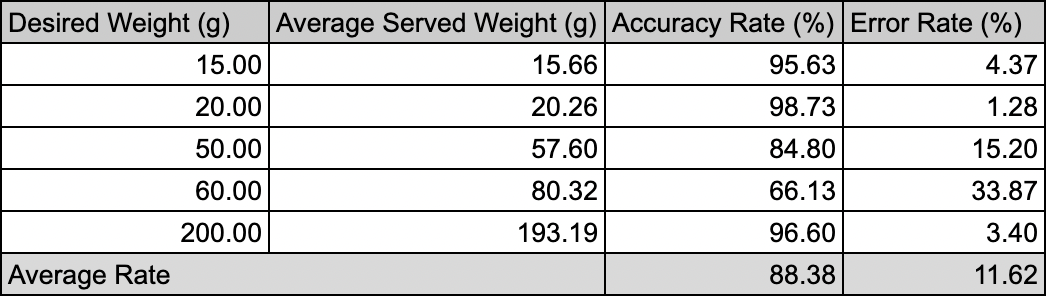
\includegraphics[width=0.5\textwidth]{./images/serve-accuracy.png}}
%\caption{Testing result of automatic feeding}
%\label{fig}
%\end{figure}
%
\begin{table}[htbp]
\caption{Testing result of automatic feeding}
\begin{center}
\begin{tabular}{|c|c|c|c|}
%\begin{tabularx}{\columnwidth}{|X|X|X|X|}
\hline
%\textbf{Table}&\multicolumn{3}{|c|}{\textbf{Table Column Head}} \\
%\cline{2-4} 
\textbf{\textit{Desired}} & \textbf{\textit{Average Served}}& \textbf{\textit{Accuracy}}& \textbf{\textit{Error}} \\
\textbf{\textit{Weight(g)}} & \textbf{\textit{Weight(g)}}& \textbf{\textit{(\%)}}& \textbf{\textit{(\%)}} \\
\hline
15.00& 15.66& 95.63 & 4.37 \\
\hline
20.00& 20.26& 98.73 & 1.28 \\
\hline
50.00& 57.60& 84.80 & 15.20 \\
\hline
60.00& 80.32& 66.13 & 33..87 \\
\hline
200.00& 193.19& 96.60 & 3.40 \\
\hline
\hline
\multicolumn{2}{|c|}{\textbf{Average Rate}}& 88.38 & 11.62 \\
\hline
\end{tabular}
\label{tab1}
\end{center}
\end{table}

\subsection{Automatic Feeding Test}
One of the features of this solution is the automatic food feeding. We evaluated the accuracy of the automatic food serving feature.
The difference between the five desired weights and the average actual served weight are compared in Table~\ref{tab1}. 
The solution has an average accuracy rate of 88.38\%.
The reason for the error is that food often gets stuck in front of the food gate, and the transfer speed is too fast for the load cell to detect.
This is due to the limitation of the feed machine and can be resolved by modifying the design of the machine.


\balance 
\section{Conclusion}
In summary, we proposed the pet-care IoT solution "Petification" that can take care of pets remotely. 
Petification supports tracking food and water consumption and remote feeding with the web-based dashboard.  
We also demonstrated that the solution provided device status information and error notification.  
The advantages of the open-source projects are to develop faster, and leverage the rich ecosystem of resources created by its users.
We expect to add more features to extend Petification by leveraging open-source advantages.
Current limitation of Petification is the relatively low accuracy of automatic food serving due to the design of the food gate and the sensitivity of the load cell.
Therefore, future work includes improving the accuracy of servings by addressing these issues.

\section*{Acknowledgment}
This research was supported by the MSIT(Ministry of Science and ICT), Korea, under the National Program for Excellence in SW) supervised by the IITP(Institute of Information \& communications Technology Planning \& Evaluation) in 2021”(2021-0-01435)

%\section*{References}

\begin{thebibliography}{00}
\bibitem{b1} 
M.  Hanson.  “Pet  Industry  Statistics”  spots.com.  https://spots.com/pet-industry-statistics/ (accessed Jan. 25, 2022). 
\bibitem{b2}
Accessed: Feb. 1, 2022. [Online]. Available: https://www.instructables.com/IOT-Pet-Feeder-Using-the-Blynk-Mobile-App-an-ESP82/
\bibitem{b3}
T. Sangvanloy and K. Sookhanaphibarn, "Automatic Pet Food Dispenser by using Internet of Things (IoT)," 2020 IEEE 2nd Global Conference on Life Sciences and Technologies (LifeTech), Kyoto, Japan, Mar. 10-12, 2020.
\bibitem{b4}
Y. Chen and M. Elshakankiri, "Implementation of an IoT based Pet Care System," 2020 Fifth International Conference on Fog and Mobile Edge Computing (FMEC), Paris, France, Apr. 20-23, 2020.
\bibitem{b5}
Accessed: Feb. 4, 2022. [Online]. Available: https://iotdesignpro.com/projects/google-assistant-controlled-iot-pet-feeder-using-esp8266
\bibitem{b6}
Accessed: Feb. 5, 2022. [Online]. Available: https://create.arduino.cc/projecthub/circuito-io-team/iot-pet-feeder-10a4f3
\bibitem{b7}
Node-RED [Online]. Available: https://nodered.org/about/
\bibitem{b11}
Vania, K. Karyono and I. H. T. Nugroho, "Smart dog feeder design using wireless communication, MQTT and Android client," 2016 International Conference on Computer, Control, Informatics and its Applications (IC3INA), Tangerang, Indonesia, Oct. 3-5, 2016.
\bibitem{b10}
R. Nogueira, H. Araújo and D. Prata. (Apr. 2019). Robot Chow: Automatic Animal Feeding with Intelligent Interface to Monitor Pets. International Journal of Advanced Engineering Research and Science. [Online]. Available: https://ijaers.com/detail/robot-chow-automatic-animal-feeding-with-intelligent-interface-to-monitor-pets/
\bibitem{b9}
P. N. Vrishanka, P. Prabhakar, D. Shet and K. Rupali, "Automated Pet Feeder using IoT," 2021 IEEE International Conference on Mobile Networks and Wireless Communications (ICMNWC), Tumkur, Karnataka, India, Dec. 3-4, 2021.
\bibitem{b8}
MQTT [Online]. Available: https://mqtt.org
\bibitem{b12}
N. B. Kamarozaman and A. H. Awang, "IOT COVID-19 Portable Health Monitoring System using Raspberry Pi, Node-Red and ThingSpeak," 2021 IEEE Symposium on Wireless Technology \& Applications (ISWTA), Shah Alam, Malaysia, Aug. 17-17, 2021.
\bibitem{b13}
Eclipse Mosquitto [Online]. Available: https://mosquitto.org/
\bibitem{b14}
A. Tamboli, “Build Your Own IoT Platform,” in \textit{Apress}, 1st ed, 2019
\end{thebibliography}

%\vspace{12pt}

\end{document}


%%%
%%
%% figure table



%\begin{figure}[htbp]
%\centerline{\includegraphics{fig1.png}}
%\caption{Example of a figure caption.}
%\label{fig}
%\end{figure}
